\documentclass[11pt, t, aspectratio=169]{beamer}
% \documentclass[11pt,compress,t,notes=noshow, xcolor=table]{beamer}
\usepackage[]{graphicx}\usepackage[]{color}
% maxwidth is the original width if it is less than linewidth
% otherwise use linewidth (to make sure the graphics do not exceed the margin)
\makeatletter
\def\maxwidth{ %
  \ifdim\Gin@nat@width>\linewidth
    \linewidth
  \else
    \Gin@nat@width
  \fi
}
\makeatother

\definecolor{fgcolor}{rgb}{0.345, 0.345, 0.345}
\newcommand{\hlnum}[1]{\textcolor[rgb]{0.686,0.059,0.569}{#1}}%
\newcommand{\hlstr}[1]{\textcolor[rgb]{0.192,0.494,0.8}{#1}}%
\newcommand{\hlcom}[1]{\textcolor[rgb]{0.678,0.584,0.686}{\textit{#1}}}%
\newcommand{\hlopt}[1]{\textcolor[rgb]{0,0,0}{#1}}%
\newcommand{\hlstd}[1]{\textcolor[rgb]{0.345,0.345,0.345}{#1}}%
\newcommand{\hlkwa}[1]{\textcolor[rgb]{0.161,0.373,0.58}{\textbf{#1}}}%
\newcommand{\hlkwb}[1]{\textcolor[rgb]{0.69,0.353,0.396}{#1}}%
\newcommand{\hlkwc}[1]{\textcolor[rgb]{0.333,0.667,0.333}{#1}}%
\newcommand{\hlkwd}[1]{\textcolor[rgb]{0.737,0.353,0.396}{\textbf{#1}}}%
\let\hlipl\hlkwb

\usepackage{framed}
\makeatletter
\newenvironment{kframe}{%
 \def\at@end@of@kframe{}%
 \ifinner\ifhmode%
  \def\at@end@of@kframe{\end{minipage}}%
  \begin{minipage}{\columnwidth}%
 \fi\fi%
 \def\FrameCommand##1{\hskip\@totalleftmargin \hskip-\fboxsep
 \colorbox{shadecolor}{##1}\hskip-\fboxsep
     % There is no \\@totalrightmargin, so:
     \hskip-\linewidth \hskip-\@totalleftmargin \hskip\columnwidth}%
 \MakeFramed {\advance\hsize-\width
   \@totalleftmargin\z@ \linewidth\hsize
   \@setminipage}}%
 {\par\unskip\endMakeFramed%
 \at@end@of@kframe}
\makeatother

\definecolor{shadecolor}{rgb}{.97, .97, .97}
\definecolor{messagecolor}{rgb}{0, 0, 0}
\definecolor{warningcolor}{rgb}{1, 0, 1}
\definecolor{errorcolor}{rgb}{1, 0, 0}
\newenvironment{knitrout}{}{} % an empty environment to be redefined in TeX

\usepackage{alltt}
\newcommand{\SweaveOpts}[1]{}  % do not interfere with LaTeX
\newcommand{\SweaveInput}[1]{} % because they are not real TeX commands
\newcommand{\Sexpr}[1]{}       % will only be parsed by R
\newcommand{\xmark}{\ding{55}}%


\usepackage[english]{babel}
\usepackage[utf8]{inputenc}

\usepackage{dsfont}
\usepackage{verbatim}
\usepackage{amsmath}
\usepackage{amsfonts}
\usepackage{amssymb}
\usepackage{bm}
\usepackage{csquotes}
\usepackage{multirow}
\usepackage{longtable}
\usepackage{booktabs}
\usepackage{enumerate}
\usepackage[absolute,overlay]{textpos}
\usepackage{psfrag}
\usepackage{algorithm}
\usepackage{algpseudocode}
\usepackage{eqnarray}
\usepackage{arydshln}
\usepackage{tabularx}
\usepackage{placeins}
\usepackage{tikz}
\usepackage{setspace}
\usepackage{colortbl}
\usepackage{mathtools}
\usepackage{wrapfig}
\usepackage{bm}
\usepackage{amsmath}
\usepackage{pifont}
\usepackage[round]{natbib}
\usepackage{hyperref}

\usetikzlibrary{shapes,arrows,automata,positioning,calc,chains,trees, shadows}
\tikzset{
  %Define standard arrow tip
  >=stealth',
  %Define style for boxes
  punkt/.style={
    rectangle,
    rounded corners,
    draw=black, very thick,
    text width=6.5em,
    minimum height=2em,
    text centered},
  % Define arrow style
  pil/.style={
    ->,
    thick,
    shorten <=2pt,
    shorten >=2pt,}
}

\usepackage{subfig}

% Defines macros and environments
\usepackage{../../style/lmu-lecture}


\let\code=\texttt
\let\proglang=\textsf

\setkeys{Gin}{width=0.9\textwidth}

\setbeamertemplate{frametitle}{\expandafter\uppercase\expandafter\insertframetitle}

% basic latex stuff
\newcommand{\pkg}[1]{{\fontseries{b}\selectfont #1}} % fontstyle for R packages

% Often used in exercise Rnw files, still relevant?
\newcommand{\lz}{\vspace{0.5cm}} % vertical space
\newcommand{\dlz}{\vspace{1cm}}  % double vertical space

% Unused and about to be deleted
\newcommand{\oneliner}[1] % Oneliner for important statements
{\begin{block}{}\begin{center}\begin{Large}#1\end{Large}\end{center}\end{block}}


%--------------------%
%  New environments  %
%--------------------%

 % Frame with breaks and verbatim // this is used very often
\newenvironment{vbframe}
{
\begin{frame}[containsverbatim,allowframebreaks]
}
{
\end{frame}
}

% Frame with verbatim without breaks (to avoid numbering one slided frames)
% This is not used anywhere but I can see it being useful
\newenvironment{vframe}
{
\begin{frame}[containsverbatim]
}
{
\end{frame}
}

% Itemize block
\newenvironment{blocki}[1]
{
\begin{block}{#1}\begin{itemize}
}
{
\end{itemize}\end{block}
}

%--------------%
%  Citebutton  %
%--------------%
% Example usage (from slides-cart-discussion.tex)
% \citebutton{Breiman, 1984}{https://www.taylorfrancis.com/books/mono/10.1201/9781315139470/classification-regression-trees-leo-breiman}
\newcommand{\citebutton}[2]{%
\NoCaseChange{\resizebox{!}{9pt}{\protect\beamergotobutton{\href{#2}{#1}}}}%
}

% textcolor that works in mathmode
% https://tex.stackexchange.com/a/261480
% Used e.g. in forests/slides-forests-bagging.tex
% [...] \textcolor{blue}{\tfrac{1}{M}\sum^M_{m} [...]
\makeatletter
\renewcommand*{\@textcolor}[3]{%
  \protect\leavevmode
  \begingroup
    \color#1{#2}#3%
  \endgroup
}
\makeatother




 % use this if compiling with make file
\documentclass[11pt,compress,t,notes=noshow, xcolor=table]{beamer}
\usepackage[]{graphicx}\usepackage[]{color}
% maxwidth is the original width if it is less than linewidth
% otherwise use linewidth (to make sure the graphics do not exceed the margin)
\makeatletter
\def\maxwidth{ %
  \ifdim\Gin@nat@width>\linewidth
    \linewidth
  \else
    \Gin@nat@width
  \fi
}
\makeatother

\definecolor{fgcolor}{rgb}{0.345, 0.345, 0.345}
\newcommand{\hlnum}[1]{\textcolor[rgb]{0.686,0.059,0.569}{#1}}%
\newcommand{\hlstr}[1]{\textcolor[rgb]{0.192,0.494,0.8}{#1}}%
\newcommand{\hlcom}[1]{\textcolor[rgb]{0.678,0.584,0.686}{\textit{#1}}}%
\newcommand{\hlopt}[1]{\textcolor[rgb]{0,0,0}{#1}}%
\newcommand{\hlstd}[1]{\textcolor[rgb]{0.345,0.345,0.345}{#1}}%
\newcommand{\hlkwa}[1]{\textcolor[rgb]{0.161,0.373,0.58}{\textbf{#1}}}%
\newcommand{\hlkwb}[1]{\textcolor[rgb]{0.69,0.353,0.396}{#1}}%
\newcommand{\hlkwc}[1]{\textcolor[rgb]{0.333,0.667,0.333}{#1}}%
\newcommand{\hlkwd}[1]{\textcolor[rgb]{0.737,0.353,0.396}{\textbf{#1}}}%
\let\hlipl\hlkwb

\usepackage{framed}
\makeatletter
\newenvironment{kframe}{%
 \def\at@end@of@kframe{}%
 \ifinner\ifhmode%
  \def\at@end@of@kframe{\end{minipage}}%
  \begin{minipage}{\columnwidth}%
 \fi\fi%
 \def\FrameCommand##1{\hskip\@totalleftmargin \hskip-\fboxsep
 \colorbox{shadecolor}{##1}\hskip-\fboxsep
     % There is no \\@totalrightmargin, so:
     \hskip-\linewidth \hskip-\@totalleftmargin \hskip\columnwidth}%
 \MakeFramed {\advance\hsize-\width
   \@totalleftmargin\z@ \linewidth\hsize
   \@setminipage}}%
 {\par\unskip\endMakeFramed%
 \at@end@of@kframe}
\makeatother

\definecolor{shadecolor}{rgb}{.97, .97, .97}
\definecolor{messagecolor}{rgb}{0, 0, 0}
\definecolor{warningcolor}{rgb}{1, 0, 1}
\definecolor{errorcolor}{rgb}{1, 0, 0}
\newenvironment{knitrout}{}{} % an empty environment to be redefined in TeX

\usepackage{alltt}
\newcommand{\SweaveOpts}[1]{}  % do not interfere with LaTeX
\newcommand{\SweaveInput}[1]{} % because they are not real TeX commands
\newcommand{\Sexpr}[1]{}       % will only be parsed by R
\newcommand{\xmark}{\ding{55}}%


\usepackage[english]{babel}
\usepackage[utf8]{inputenc}

\usepackage{dsfont}
\usepackage{verbatim}
\usepackage{amsmath}
\usepackage{amsfonts}
\usepackage{amssymb}
\usepackage{bm}
\usepackage{csquotes}
\usepackage{multirow}
\usepackage{longtable}
\usepackage{booktabs}
\usepackage{enumerate}
\usepackage[absolute,overlay]{textpos}
\usepackage{psfrag}
\usepackage{algorithm}
\usepackage{algpseudocode}
\usepackage{eqnarray}
\usepackage{arydshln}
\usepackage{tabularx}
\usepackage{placeins}
\usepackage{tikz}
\usepackage{setspace}
\usepackage{colortbl}
\usepackage{mathtools}
\usepackage{wrapfig}
\usepackage{bm}
\usepackage{amsmath}
\usepackage{pifont}
\usepackage[round]{natbib}
\usepackage{hyperref}

\usetikzlibrary{shapes,arrows,automata,positioning,calc,chains,trees, shadows}
\tikzset{
  %Define standard arrow tip
  >=stealth',
  %Define style for boxes
  punkt/.style={
    rectangle,
    rounded corners,
    draw=black, very thick,
    text width=6.5em,
    minimum height=2em,
    text centered},
  % Define arrow style
  pil/.style={
    ->,
    thick,
    shorten <=2pt,
    shorten >=2pt,}
}

\usepackage{subfig}

% Defines macros and environments
\usepackage{../../style/lmu-lecture}


\let\code=\texttt
\let\proglang=\textsf

\setkeys{Gin}{width=0.9\textwidth}

\setbeamertemplate{frametitle}{\expandafter\uppercase\expandafter\insertframetitle}

% basic latex stuff
\newcommand{\pkg}[1]{{\fontseries{b}\selectfont #1}} % fontstyle for R packages

% Often used in exercise Rnw files, still relevant?
\newcommand{\lz}{\vspace{0.5cm}} % vertical space
\newcommand{\dlz}{\vspace{1cm}}  % double vertical space

% Unused and about to be deleted
\newcommand{\oneliner}[1] % Oneliner for important statements
{\begin{block}{}\begin{center}\begin{Large}#1\end{Large}\end{center}\end{block}}


%--------------------%
%  New environments  %
%--------------------%

 % Frame with breaks and verbatim // this is used very often
\newenvironment{vbframe}
{
\begin{frame}[containsverbatim,allowframebreaks]
}
{
\end{frame}
}

% Frame with verbatim without breaks (to avoid numbering one slided frames)
% This is not used anywhere but I can see it being useful
\newenvironment{vframe}
{
\begin{frame}[containsverbatim]
}
{
\end{frame}
}

% Itemize block
\newenvironment{blocki}[1]
{
\begin{block}{#1}\begin{itemize}
}
{
\end{itemize}\end{block}
}

%--------------%
%  Citebutton  %
%--------------%
% Example usage (from slides-cart-discussion.tex)
% \citebutton{Breiman, 1984}{https://www.taylorfrancis.com/books/mono/10.1201/9781315139470/classification-regression-trees-leo-breiman}
\newcommand{\citebutton}[2]{%
\NoCaseChange{\resizebox{!}{9pt}{\protect\beamergotobutton{\href{#2}{#1}}}}%
}

% textcolor that works in mathmode
% https://tex.stackexchange.com/a/261480
% Used e.g. in forests/slides-forests-bagging.tex
% [...] \textcolor{blue}{\tfrac{1}{M}\sum^M_{m} [...]
\makeatletter
\renewcommand*{\@textcolor}[3]{%
  \protect\leavevmode
  \begingroup
    \color#1{#2}#3%
  \endgroup
}
\makeatother




 % use this if compiling in overleaf
% dependencies: amsmath, amssymb, dsfont
% math spaces
\ifdefined\N
\renewcommand{\N}{\mathds{N}} % N, naturals
\else \newcommand{\N}{\mathds{N}} \fi
\newcommand{\Z}{\mathds{Z}} % Z, integers
\newcommand{\Q}{\mathds{Q}} % Q, rationals
\newcommand{\R}{\mathds{R}} % R, reals
\ifdefined\C
\renewcommand{\C}{\mathds{C}} % C, complex
\else \newcommand{\C}{\mathds{C}} \fi
\newcommand{\continuous}{\mathcal{C}} % C, space of continuous functions
\newcommand{\M}{\mathcal{M}} % machine numbers
\newcommand{\epsm}{\epsilon_m} % maximum error

% counting / finite sets
\newcommand{\setzo}{\{0, 1\}} % set 0, 1
\newcommand{\setmp}{\{-1, +1\}} % set -1, 1
\newcommand{\unitint}{[0, 1]} % unit interval

% basic math stuff
\newcommand{\xt}{\tilde x} % x tilde
\DeclareMathOperator*{\argmax}{arg\,max} % argmax
\DeclareMathOperator*{\argmin}{arg\,min} % argmin
\newcommand{\argminlim}{\mathop{\mathrm{arg\,min}}\limits} % argmax with limits
\newcommand{\argmaxlim}{\mathop{\mathrm{arg\,max}}\limits} % argmin with limits
\newcommand{\sign}{\operatorname{sign}} % sign, signum
\newcommand{\I}{\mathbb{I}} % I, indicator
\newcommand{\order}{\mathcal{O}} % O, order
\newcommand{\bigO}{\mathcal{O}} % Big-O Landau
\newcommand{\littleo}{{o}} % Little-o Landau
\newcommand{\pd}[2]{\frac{\partial{#1}}{\partial #2}} % partial derivative
\newcommand{\floorlr}[1]{\left\lfloor #1 \right\rfloor} % floor
\newcommand{\ceillr}[1]{\left\lceil #1 \right\rceil} % ceiling
\newcommand{\indep}{\perp \!\!\! \perp} % independence symbol

% sums and products
\newcommand{\sumin}{\sum\limits_{i=1}^n} % summation from i=1 to n
\newcommand{\sumim}{\sum\limits_{i=1}^m} % summation from i=1 to m
\newcommand{\sumjn}{\sum\limits_{j=1}^n} % summation from j=1 to p
\newcommand{\sumjp}{\sum\limits_{j=1}^p} % summation from j=1 to p
\newcommand{\sumik}{\sum\limits_{i=1}^k} % summation from i=1 to k
\newcommand{\sumkg}{\sum\limits_{k=1}^g} % summation from k=1 to g
\newcommand{\sumjg}{\sum\limits_{j=1}^g} % summation from j=1 to g
\newcommand{\meanin}{\frac{1}{n} \sum\limits_{i=1}^n} % mean from i=1 to n
\newcommand{\meanim}{\frac{1}{m} \sum\limits_{i=1}^m} % mean from i=1 to n
\newcommand{\meankg}{\frac{1}{g} \sum\limits_{k=1}^g} % mean from k=1 to g
\newcommand{\prodin}{\prod\limits_{i=1}^n} % product from i=1 to n
\newcommand{\prodkg}{\prod\limits_{k=1}^g} % product from k=1 to g
\newcommand{\prodjp}{\prod\limits_{j=1}^p} % product from j=1 to p

% linear algebra
\newcommand{\one}{\bm{1}} % 1, unitvector
\newcommand{\zero}{\mathbf{0}} % 0-vector
\newcommand{\id}{\bm{I}} % I, identity
\newcommand{\diag}{\operatorname{diag}} % diag, diagonal
\newcommand{\trace}{\operatorname{tr}} % tr, trace
\newcommand{\spn}{\operatorname{span}} % span
\newcommand{\scp}[2]{\left\langle #1, #2 \right\rangle} % <.,.>, scalarproduct
\newcommand{\mat}[1]{\begin{pmatrix} #1 \end{pmatrix}} % short pmatrix command
\newcommand{\Amat}{\mathbf{A}} % matrix A
\newcommand{\Deltab}{\mathbf{\Delta}} % error term for vectors

% basic probability + stats
\renewcommand{\P}{\mathds{P}} % P, probability
\newcommand{\E}{\mathds{E}} % E, expectation
\newcommand{\var}{\mathsf{Var}} % Var, variance
\newcommand{\cov}{\mathsf{Cov}} % Cov, covariance
\newcommand{\corr}{\mathsf{Corr}} % Corr, correlation
\newcommand{\normal}{\mathcal{N}} % N of the normal distribution
\newcommand{\iid}{\overset{i.i.d}{\sim}} % dist with i.i.d superscript
\newcommand{\distas}[1]{\overset{#1}{\sim}} % ... is distributed as ...

% machine learning
\newcommand{\Xspace}{\mathcal{X}} % X, input space
\newcommand{\Yspace}{\mathcal{Y}} % Y, output space
\newcommand{\Zspace}{\mathcal{Z}} % Z, space of sampled datapoints
\newcommand{\nset}{\{1, \ldots, n\}} % set from 1 to n
\newcommand{\pset}{\{1, \ldots, p\}} % set from 1 to p
\newcommand{\gset}{\{1, \ldots, g\}} % set from 1 to g
\newcommand{\Pxy}{\mathbb{P}_{xy}} % P_xy
\newcommand{\Exy}{\mathbb{E}_{xy}} % E_xy: Expectation over random variables xy
\newcommand{\xv}{\mathbf{x}} % vector x (bold)
\newcommand{\xtil}{\tilde{\mathbf{x}}} % vector x-tilde (bold)
\newcommand{\yv}{\mathbf{y}} % vector y (bold)
\newcommand{\xy}{(\xv, y)} % observation (x, y)
\newcommand{\xvec}{\left(x_1, \ldots, x_p\right)^\top} % (x1, ..., xp)
\newcommand{\Xmat}{\mathbf{X}} % Design matrix
\newcommand{\allDatasets}{\mathds{D}} % The set of all datasets
\newcommand{\allDatasetsn}{\mathds{D}_n}  % The set of all datasets of size n
\newcommand{\D}{\mathcal{D}} % D, data
\newcommand{\Dn}{\D_n} % D_n, data of size n
\newcommand{\Dtrain}{\mathcal{D}_{\text{train}}} % D_train, training set
\newcommand{\Dtest}{\mathcal{D}_{\text{test}}} % D_test, test set
\newcommand{\xyi}[1][i]{\left(\xv^{(#1)}, y^{(#1)}\right)} % (x^i, y^i), i-th observation
\newcommand{\Dset}{\left( \xyi[1], \ldots, \xyi[n]\right)} % {(x1,y1)), ..., (xn,yn)}, data
\newcommand{\defAllDatasetsn}{(\Xspace \times \Yspace)^n} % Def. of the set of all datasets of size n
\newcommand{\defAllDatasets}{\bigcup_{n \in \N}(\Xspace \times \Yspace)^n} % Def. of the set of all datasets
\newcommand{\xdat}{\left\{ \xv^{(1)}, \ldots, \xv^{(n)}\right\}} % {x1, ..., xn}, input data
\newcommand{\ydat}{\left\{ \yv^{(1)}, \ldots, \yv^{(n)}\right\}} % {y1, ..., yn}, input data
\newcommand{\yvec}{\left(y^{(1)}, \hdots, y^{(n)}\right)^\top} % (y1, ..., yn), vector of outcomes
\newcommand{\greekxi}{\xi} % Greek letter xi
\renewcommand{\xi}[1][i]{\xv^{(#1)}} % x^i, i-th observed value of x
\newcommand{\yi}[1][i]{y^{(#1)}} % y^i, i-th observed value of y
\newcommand{\xivec}{\left(x^{(i)}_1, \ldots, x^{(i)}_p\right)^\top} % (x1^i, ..., xp^i), i-th observation vector
\newcommand{\xj}{\xv_j} % x_j, j-th feature
\newcommand{\xjvec}{\left(x^{(1)}_j, \ldots, x^{(n)}_j\right)^\top} % (x^1_j, ..., x^n_j), j-th feature vector
\newcommand{\phiv}{\mathbf{\phi}} % Basis transformation function phi
\newcommand{\phixi}{\mathbf{\phi}^{(i)}} % Basis transformation of xi: phi^i := phi(xi)

%%%%%% ml - models general
\newcommand{\lamv}{\bm{\lambda}} % lambda vector, hyperconfiguration vector
\newcommand{\Lam}{\bm{\Lambda}}	 % Lambda, space of all hpos
% Inducer / Inducing algorithm
\newcommand{\preimageInducer}{\left(\defAllDatasets\right)\times\Lam} % Set of all datasets times the hyperparameter space
\newcommand{\preimageInducerShort}{\allDatasets\times\Lam} % Set of all datasets times the hyperparameter space
% Inducer / Inducing algorithm
\newcommand{\ind}{\mathcal{I}} % Inducer, inducing algorithm, learning algorithm

% continuous prediction function f
\newcommand{\ftrue}{f_{\text{true}}}  % True underlying function (if a statistical model is assumed)
\newcommand{\ftruex}{\ftrue(\xv)} % True underlying function (if a statistical model is assumed)
\newcommand{\fx}{f(\xv)} % f(x), continuous prediction function
\newcommand{\fdomains}{f: \Xspace \rightarrow \R^g} % f with domain and co-domain
\newcommand{\Hspace}{\mathcal{H}} % hypothesis space where f is from
\newcommand{\fbayes}{f^{\ast}} % Bayes-optimal model
\newcommand{\fxbayes}{f^{\ast}(\xv)} % Bayes-optimal model
\newcommand{\fkx}[1][k]{f_{#1}(\xv)} % f_j(x), discriminant component function
\newcommand{\fh}{\hat{f}} % f hat, estimated prediction function
\newcommand{\fxh}{\fh(\xv)} % fhat(x)
\newcommand{\fxt}{f(\xv ~|~ \thetav)} % f(x | theta)
\newcommand{\fxi}{f\left(\xv^{(i)}\right)} % f(x^(i))
\newcommand{\fxih}{\hat{f}\left(\xv^{(i)}\right)} % f(x^(i))
\newcommand{\fxit}{f\left(\xv^{(i)} ~|~ \thetav\right)} % f(x^(i) | theta)
\newcommand{\fhD}{\fh_{\D}} % fhat_D, estimate of f based on D
\newcommand{\fhDtrain}{\fh_{\Dtrain}} % fhat_Dtrain, estimate of f based on D
\newcommand{\fhDnlam}{\fh_{\Dn, \lamv}} %model learned on Dn with hp lambda
\newcommand{\fhDlam}{\fh_{\D, \lamv}} %model learned on D with hp lambda
\newcommand{\fhDnlams}{\fh_{\Dn, \lamv^\ast}} %model learned on Dn with optimal hp lambda
\newcommand{\fhDlams}{\fh_{\D, \lamv^\ast}} %model learned on D with optimal hp lambda

% discrete prediction function h
\newcommand{\hx}{h(\xv)} % h(x), discrete prediction function
\newcommand{\hh}{\hat{h}} % h hat
\newcommand{\hxh}{\hat{h}(\xv)} % hhat(x)
\newcommand{\hxt}{h(\xv | \thetav)} % h(x | theta)
\newcommand{\hxi}{h\left(\xi\right)} % h(x^(i))
\newcommand{\hxit}{h\left(\xi ~|~ \thetav\right)} % h(x^(i) | theta)
\newcommand{\hbayes}{h^{\ast}} % Bayes-optimal classification model
\newcommand{\hxbayes}{h^{\ast}(\xv)} % Bayes-optimal classification model

% yhat
\newcommand{\yh}{\hat{y}} % yhat for prediction of target
\newcommand{\yih}{\hat{y}^{(i)}} % yhat^(i) for prediction of ith targiet
\newcommand{\resi}{\yi- \yih}

% theta
\newcommand{\thetah}{\hat{\theta}} % theta hat
\newcommand{\thetav}{\bm{\theta}} % theta vector
\newcommand{\thetavh}{\bm{\hat\theta}} % theta vector hat
\newcommand{\thetat}[1][t]{\thetav^{[#1]}} % theta^[t] in optimization
\newcommand{\thetatn}[1][t]{\thetav^{[#1 +1]}} % theta^[t+1] in optimization
\newcommand{\thetahDnlam}{\thetavh_{\Dn, \lamv}} %theta learned on Dn with hp lambda
\newcommand{\thetahDlam}{\thetavh_{\D, \lamv}} %theta learned on D with hp lambda
\newcommand{\mint}{\min_{\thetav \in \Theta}} % min problem theta
\newcommand{\argmint}{\argmin_{\thetav \in \Theta}} % argmin theta

% densities + probabilities
% pdf of x
\newcommand{\pdf}{p} % p
\newcommand{\pdfx}{p(\xv)} % p(x)
\newcommand{\pixt}{\pi(\xv~|~ \thetav)} % pi(x|theta), pdf of x given theta
\newcommand{\pixit}[1][i]{\pi\left(\xi[#1] ~|~ \thetav\right)} % pi(x^i|theta), pdf of x given theta
\newcommand{\pixii}[1][i]{\pi\left(\xi[#1]\right)} % pi(x^i), pdf of i-th x

% pdf of (x, y)
\newcommand{\pdfxy}{p(\xv,y)} % p(x, y)
\newcommand{\pdfxyt}{p(\xv, y ~|~ \thetav)} % p(x, y | theta)
\newcommand{\pdfxyit}{p\left(\xi, \yi ~|~ \thetav\right)} % p(x^(i), y^(i) | theta)

% pdf of x given y
\newcommand{\pdfxyk}[1][k]{p(\xv | y= #1)} % p(x | y = k)
\newcommand{\lpdfxyk}[1][k]{\log p(\xv | y= #1)} % log p(x | y = k)
\newcommand{\pdfxiyk}[1][k]{p\left(\xi | y= #1 \right)} % p(x^i | y = k)

% prior probabilities
\newcommand{\pik}[1][k]{\pi_{#1}} % pi_k, prior
\newcommand{\lpik}[1][k]{\log \pi_{#1}} % log pi_k, log of the prior
\newcommand{\pit}{\pi(\thetav)} % Prior probability of parameter theta

% posterior probabilities
\newcommand{\post}{\P(y = 1 ~|~ \xv)} % P(y = 1 | x), post. prob for y=1
\newcommand{\postk}[1][k]{\P(y = #1 ~|~ \xv)} % P(y = k | y), post. prob for y=k
\newcommand{\pidomains}{\pi: \Xspace \rightarrow \unitint} % pi with domain and co-domain
\newcommand{\pibayes}{\pi^{\ast}} % Bayes-optimal classification model
\newcommand{\pixbayes}{\pi^{\ast}(\xv)} % Bayes-optimal classification model
\newcommand{\pix}{\pi(\xv)} % pi(x), P(y = 1 | x)
\newcommand{\piv}{\bm{\pi}} % pi, bold, as vector
\newcommand{\pikx}[1][k]{\pi_{#1}(\xv)} % pi_k(x), P(y = k | x)
\newcommand{\pikxt}[1][k]{\pi_{#1}(\xv ~|~ \thetav)} % pi_k(x | theta), P(y = k | x, theta)
\newcommand{\pixh}{\hat \pi(\xv)} % pi(x) hat, P(y = 1 | x) hat
\newcommand{\pikxh}[1][k]{\hat \pi_{#1}(\xv)} % pi_k(x) hat, P(y = k | x) hat
\newcommand{\pixih}{\hat \pi(\xi)} % pi(x^(i)) with hat
\newcommand{\pikxih}[1][k]{\hat \pi_{#1}(\xi)} % pi_k(x^(i)) with hat
\newcommand{\pdfygxt}{p(y ~|~\xv, \thetav)} % p(y | x, theta)
\newcommand{\pdfyigxit}{p\left(\yi ~|~\xi, \thetav\right)} % p(y^i |x^i, theta)
\newcommand{\lpdfygxt}{\log \pdfygxt } % log p(y | x, theta)
\newcommand{\lpdfyigxit}{\log \pdfyigxit} % log p(y^i |x^i, theta)

% probababilistic
\newcommand{\bayesrulek}[1][k]{\frac{\P(\xv | y= #1) \P(y= #1)}{\P(\xv)}} % Bayes rule
\newcommand{\muk}{\bm{\mu_k}} % mean vector of class-k Gaussian (discr analysis)

% residual and margin
\newcommand{\eps}{\epsilon} % residual, stochastic
\newcommand{\epsv}{\bm{\epsilon}} % residual, stochastic, as vector
\newcommand{\epsi}{\epsilon^{(i)}} % epsilon^i, residual, stochastic
\newcommand{\epsh}{\hat{\epsilon}} % residual, estimated
\newcommand{\epsvh}{\hat{\epsv}} % residual, estimated, vector
\newcommand{\yf}{y \fx} % y f(x), margin
\newcommand{\yfi}{\yi \fxi} % y^i f(x^i), margin
\newcommand{\Sigmah}{\hat \Sigma} % estimated covariance matrix
\newcommand{\Sigmahj}{\hat \Sigma_j} % estimated covariance matrix for the j-th class

% ml - loss, risk, likelihood
\newcommand{\Lyf}{L\left(y, f\right)} % L(y, f), loss function
\newcommand{\Lypi}{L\left(y, \pi\right)} % L(y, pi), loss function
\newcommand{\Lxy}{L\left(y, \fx\right)} % L(y, f(x)), loss function
\newcommand{\Lxyi}{L\left(\yi, \fxi\right)} % loss of observation
\newcommand{\Lxyt}{L\left(y, \fxt\right)} % loss with f parameterized
\newcommand{\Lxyit}{L\left(\yi, \fxit\right)} % loss of observation with f parameterized
\newcommand{\Lxym}{L\left(\yi, f\left(\bm{\tilde{x}}^{(i)} ~|~ \thetav\right)\right)} % loss of observation with f parameterized
\newcommand{\Lpixy}{L\left(y, \pix\right)} % loss in classification
\newcommand{\Lpiv}{L\left(y, \piv\right)} % loss in classification
\newcommand{\Lpixyi}{L\left(\yi, \pixii\right)} % loss of observation in classification
\newcommand{\Lpixyt}{L\left(y, \pixt\right)} % loss with pi parameterized
\newcommand{\Lpixyit}{L\left(\yi, \pixit\right)} % loss of observation with pi parameterized
\newcommand{\Lhxy}{L\left(y, \hx\right)} % L(y, h(x)), loss function on discrete classes
\newcommand{\Lr}{L\left(r\right)} % L(r), loss defined on residual (reg) / margin (classif)
\newcommand{\lone}{|y - \fx|} % L1 loss
\newcommand{\ltwo}{\left(y - \fx\right)^2} % L2 loss
\newcommand{\lbernoullimp}{\ln(1 + \exp(-y \cdot \fx))} % Bernoulli loss for -1, +1 encoding
\newcommand{\lbernoullizo}{- y \cdot \fx + \log(1 + \exp(\fx))} % Bernoulli loss for 0, 1 encoding
\newcommand{\lcrossent}{- y \log \left(\pix\right) - (1 - y) \log \left(1 - \pix\right)} % cross-entropy loss
\newcommand{\lbrier}{\left(\pix - y \right)^2} % Brier score
\newcommand{\risk}{\mathcal{R}} % R, risk
\newcommand{\riskbayes}{\mathcal{R}^\ast}
\newcommand{\riskf}{\risk(f)} % R(f), risk
\newcommand{\riskdef}{\E_{y|\xv}\left(\Lxy \right)} % risk def (expected loss)
\newcommand{\riskt}{\mathcal{R}(\thetav)} % R(theta), risk
\newcommand{\riske}{\mathcal{R}_{\text{emp}}} % R_emp, empirical risk w/o factor 1 / n
\newcommand{\riskeb}{\bar{\mathcal{R}}_{\text{emp}}} % R_emp, empirical risk w/ factor 1 / n
\newcommand{\riskef}{\riske(f)} % R_emp(f)
\newcommand{\risket}{\mathcal{R}_{\text{emp}}(\thetav)} % R_emp(theta)
\newcommand{\riskr}{\mathcal{R}_{\text{reg}}} % R_reg, regularized risk
\newcommand{\riskrt}{\mathcal{R}_{\text{reg}}(\thetav)} % R_reg(theta)
\newcommand{\riskrf}{\riskr(f)} % R_reg(f)
\newcommand{\riskrth}{\hat{\mathcal{R}}_{\text{reg}}(\thetav)} % hat R_reg(theta)
\newcommand{\risketh}{\hat{\mathcal{R}}_{\text{emp}}(\thetav)} % hat R_emp(theta)
\newcommand{\LL}{\mathcal{L}} % L, likelihood
\newcommand{\LLt}{\mathcal{L}(\thetav)} % L(theta), likelihood
\newcommand{\LLtx}{\mathcal{L}(\thetav | \xv)} % L(theta|x), likelihood
\newcommand{\logl}{\ell} % l, log-likelihood
\newcommand{\loglt}{\logl(\thetav)} % l(theta), log-likelihood
\newcommand{\logltx}{\logl(\thetav | \xv)} % l(theta|x), log-likelihood
\newcommand{\errtrain}{\text{err}_{\text{train}}} % training error
\newcommand{\errtest}{\text{err}_{\text{test}}} % test error
\newcommand{\errexp}{\overline{\text{err}_{\text{test}}}} % avg training error

% lm
\newcommand{\thx}{\thetav^\top \xv} % linear model
\newcommand{\olsest}{(\Xmat^\top \Xmat)^{-1} \Xmat^\top \yv} % OLS estimator in LM

% linear svm
\newcommand{\sv}{\operatorname{SV}} % supportvectors
\renewcommand{\sl}{\zeta} % slack variable
\newcommand{\slvec}{\left(\zeta^{(1)}, \zeta^{(n)}\right)} % slack variable vector
\newcommand{\sli}[1][i]{\zeta^{(#1)}} % i-th slack variable
\newcommand{\scptxi}{\scp{\thetav}{\xi}} % scalar prodct of theta and xi
\newcommand{\svmhplane}{\yi \left( \scp{\thetav}{\xi} + \theta_0 \right)} % SVM hyperplane (normalized)
\newcommand{\alphah}{\hat{\alpha}} % alpha-hat (basis fun coefficients)
\newcommand{\alphav}{\bm{\alpha}} % vector alpha (bold) (basis fun coefficients)
\newcommand{\alphavh}{\hat{\bm{\alpha}}} % vector alpha-hat (basis fun coefficients)
\newcommand{\dualobj}{\sumin \alpha_i - \frac{1}{2}\sumin \sumjn \alpha_i\alpha_j\yi \yi[j] \scp{\xi}{\xv^{(j)}}} % min objective in lin svm dual

% nonlinear svm
\newcommand{\HS}{\Phi} % H, hilbertspace
\newcommand{\phix}{\phi(\xv)} % feature map x
\newcommand{\phixt}{\phi(\tilde \xv)} % feature map x tilde
\newcommand{\kxxt}{k(\xv, \tilde \xv)} % kernel fun x, x tilde
\newcommand{\scptxifm}{\scp{\thetav}{\phi(\xi)}} % scalar prodct of theta and xi

% ml - trees, extra trees

\newcommand{\Np}{\mathcal{N}} % (Parent) node N
\newcommand{\Npk}{\Np_k} % node N_k
\newcommand{\Nl}{\Np_1}	% Left node N_1
\newcommand{\Nr}{\Np_2} % Right node N_2
\newcommand{\pikN}[1][k]{\pi_#1^{(\Np)}} % class probability node N
\newcommand{\pikNh}[1][k]{\hat\pi_#1^{(\Np)}} % estimated class probability node N
\newcommand{\pikNlh}[1][k]{\hat\pi_#1^{(\Nl)}} % estimated class probability left node
\newcommand{\pikNrh}[1][k]{\hat\pi_#1^{(\Nr)}} % estimated class probability right node

% ml - bagging, random forest
\newcommand{\bl}[1][m]{b^{[#1]}} % baselearner, default m
\newcommand{\blh}[1][m]{\hat{b}^{[#1]}} % estimated base learner, default m 
\newcommand{\blx}[1][m]{b^{[#1]}(\xv)} % baselearner, default m
\newcommand{\fM}{f^{[M]}(\xv)} % ensembled predictor
\newcommand{\fMh}{\hat f^{[M]}(\xv)} % estimated ensembled predictor
\newcommand{\ambifM}{\Delta\left(\fM\right)} % ambiguity/instability of ensemble
\newcommand{\betam}[1][m]{\beta^{[#1]}} % weight of basemodel m
\newcommand{\betamh}[1][m]{\hat{\beta}^{[#1]}} % weight of basemodel m with hat
\newcommand{\betaM}{\beta^{[M]}} % last baselearner

% ml - boosting
\newcommand{\fm}[1][m]{f^{[#1]}} % prediction in iteration m
\newcommand{\fmh}[1][m]{\hat{f}^{[#1]}} % prediction in iteration m
\newcommand{\fmd}[1][m]{f^{[#1-1]}} % prediction m-1
\newcommand{\fmdh}[1][m]{\hat{f}^{[#1-1]}} % prediction m-1
\newcommand{\errm}[1][m]{\text{err}^{[#1]}} % weighted in-sample misclassification rate
\newcommand{\wm}[1][m]{w^{[#1]}} % weight vector of basemodel m
\newcommand{\wmi}[1][m]{w^{[#1](i)}} % weight of obs i of basemodel m
\newcommand{\thetam}[1][m]{\thetab^{[#1]}} % parameters of basemodel m
\newcommand{\thetamh}[1][m]{\hat{\thetab}^{[#1]}} % parameters of basemodel m with hat
\newcommand{\blxt}[1][m]{b(\xv, \thetab^{[#1]})} % baselearner, default m
\newcommand{\ens}{\sum_{m=1}^M \betam \blxt} % ensemble
\newcommand{\rmm}[1][m]{\tilde{r}^{[#1]}} % pseudo residuals
\newcommand{\rmi}[1][m]{\tilde{r}^{[#1](i)}} % pseudo residuals
\newcommand{\Rtm}[1][m]{R_{t}^{[#1]}} % terminal-region
\newcommand{\Tm}[1][m]{T^{[#1]}} % terminal-region
\newcommand{\ctm}[1][m]{c_t^{[#1]}} % mean, terminal-regions
\newcommand{\ctmh}[1][m]{\hat{c}_t^{[#1]}} % mean, terminal-regions with hat
\newcommand{\ctmt}[1][m]{\tilde{c}_t^{[#1]}} % mean, terminal-regions
\newcommand{\Lp}{L^\prime}
\newcommand{\Ldp}{L^{\prime\prime}}
\newcommand{\Lpleft}{\Lp_{\text{left}}}
\title{Important Learning Algorithms in ML}
\institute{\href{https://compstat-lmu.github.io/lecture_i2ml/}{
compstat-lmu.github.io/lecture\_i2ml}}
\author{LMU SLDS}
\date{}

% Define: \titlefigure, \titlefiguresize (as share of textwidth), 
% \titlefiguresource
\newcommand{\titlefigure}{figure_man/titlefig}
\newcommand{\titlefiguresize}{1}
\newcommand{\titlefiguresource}{https://www.keysight.com/}
\newcommand{\learninggoals}{
  \item General idea of important ML algorithms
  \item Overview of strengths and weaknesses
  % \item Understand general idea of most important ML algorithms
  % \item Learn to choose best-suited algorithm by weighing strengths and 
  % weaknesses
  % \item Apply algorithms more effectively
}

% ------------------------------------------------------------------------------

\begin{document}

\lecturechapter{}
\lecture{Introduction to Machine Learning}

\begin{frame}{Contents}
  \tableofcontents
\end{frame}

\footnotesize

%\setdraft

\section{$k$-Nearest Neighbors ($k$-NN)}
\begin{frame}{$k$-NN -- method summary}

% \maketag{Supervised} 
\maketag{regression} \maketag{classification}
\maketag{Nonparametric} \maketag{White-box}

\medskip

\highlight{General idea}
\begin{itemize}
  \item Rationale: \textbf{similarity} in feature space $\leadsto$ similarity 
  in target space w.r.t. certain \textbf{metric}
  % \item The \textbf{$k$-nearest neighbors ($k$-NN)} model is based on 
  % inter-observational \textbf{distances}, thus heavily depending on the chosen 
  % \textbf{distance measure}.
  \item \textbf{Prediction} for $\xv$: construct \textbf{$k$-neighborhood} 
  $N_k(\xv)$ from $k$ points closest to $\xv$ in $\Xspace$, then 
  predict
  \begin{itemize}
    \footnotesize
    \item (weighted) mean target for \textbf{regression}: $\yh = 1 / 
    (\sum_{i: \xi \in N_k(\xv)} w_i) \sum_{i: \xi \in N_k(\xv)} w_i \yi$
    \item most frequent class for \textbf{classification}: 
    $\yh = \argmax_{\ell \in \gset} \sum_{i: \xi \in N_k(\xv)} \I(\yi = \ell)$
  \end{itemize}
  \item No distributional or functional \textbf{assumptions}
  \item \textbf{Nonparametric} behavior: parameters = training data; no 
  compression of information
\end{itemize}

\medskip

\highlight{Hyperparameters} ~~ Neighborhood \textbf{size} $k$ (locality), 
\textbf{distance} measure

\vfill

\begin{minipage}{0.7\textwidth}
  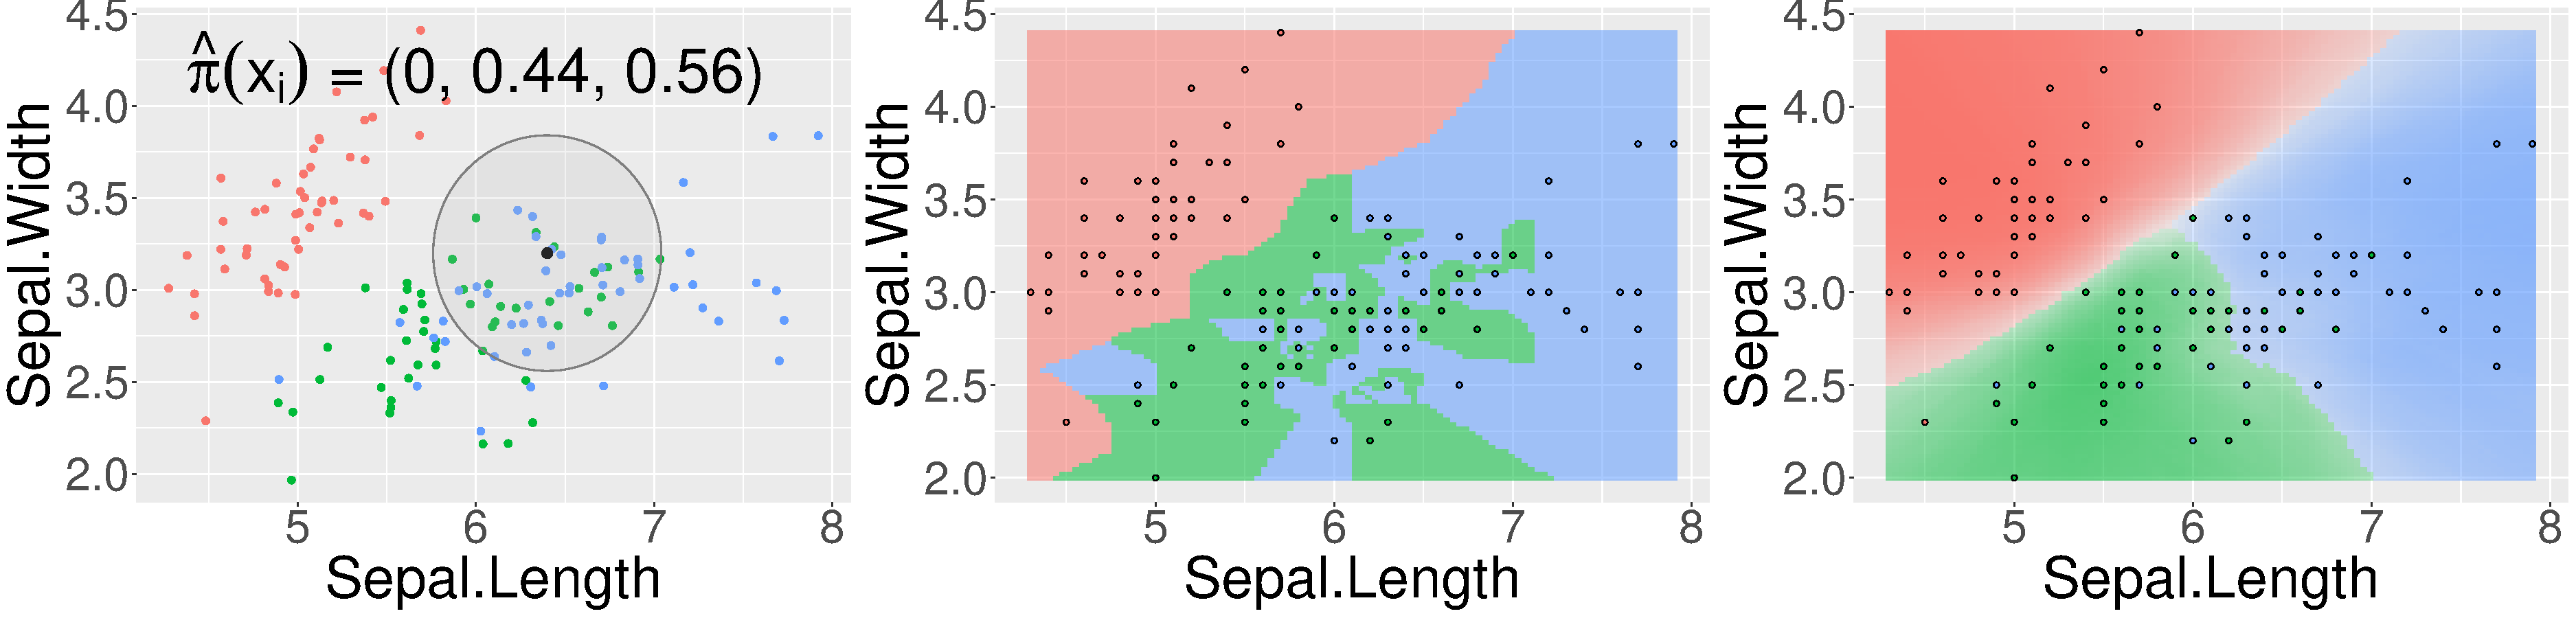
\includegraphics[width=\textwidth]{figure/knn-neighborhood.pdf}
\end{minipage}%
\hfill
\begin{minipage}{0.25\textwidth}
  \tiny
  \raggedright
  \textit{Left}: Neighborhood for exemplary observation in \texttt{iris}, 
  $k = 50$ \\
  \textit{Right}: Prediction surfaces for $k \in \{1, 50\}$
\end{minipage}
\end{frame}

% ------------------------------------------------------------------------------

\begin{frame}{$k$-NN -- Pro's \& Con's}

\footnotesize

\begin{columns}[onlytextwidth]
  \begin{column}{0.5\textwidth}
    \highlight{Advantages}
    \footnotesize
    \begin{itemize}
      \positem \textbf{Easy} to explain and implement
      % \positem Applicable to both regression and classification
      \positem No functional \textbf{assumptions} -- therefore (in theory) able 
      to model data situations of \textbf{arbitrary complexity}
      \positem No \textbf{training} period
      \positem No \textbf{optimization} required 
      \positem Constant evolvement with \textbf{new data}
      \positem Ability to learn \textbf{nonlinear} decision boundaries
      \positem Easy to \textbf{tune}
      % \positem Only one \textbf{hyperparameter} to tune
    \end{itemize}
  \end{column}
  \begin{column}{0.5\textwidth}
    \highlight{Disadvantages}
    \footnotesize
    \begin{itemize}
      \negitem Sensitivity w.r.t. \textbf{noisy} or \textbf{irrelevant} features
      and outliers due to utter reliance on distances
      \negitem Bad performance when feature \textbf{scales} not consistent 
      with importance
      \negitem Heavily afflicted by \textbf{curse of dimensionality}
      \negitem No handling of \textbf{missing} data
      \negitem Poor handling of data \textbf{imbalances} (worse for more global 
      model, i.e., large $k$)
      \negitem High \textbf{memory} consumption of distance computation
    \end{itemize}
  \end{column}
\end{columns}

\vfill

\small

\conclbox{Easy and intuitive for small, well-behaved datasets with meaningful 
feature space distances}

\end{frame}

% ------------------------------------------------------------------------------

\begin{frame}{$k$-NN -- Practical hints}

\highlight{Popular distance measures}

\begin{itemize}
  \item Numerical features: typically, \textbf{Minkowski} distances
  $d(\xv, \xtil) = \|\xv - \xtil \|_q = 
  \left( \sum_j | x_j - \tilde{x_j} |^q
  \right)^{\tfrac{1}{q}}$
  \begin{itemize}
    \item $q = 1$: \textbf{Manhattan} distance $\rightarrow d(\xv, \xtil) =
    \sum_j | x_j - \tilde{x_j} |$
  \item $q = 2$: \textbf{Euclidean} distance $\rightarrow d(\xv, \xtil) =
  \sqrt{\sum_j (x_j - \tilde{x_j})^2}$
  \end{itemize}
  \item In presence of categorical features: \textbf{Gower} distance
  \item \textbf{Custom} distance measures applicable
  \item Optional \textbf{weighting} to account for beliefs about varying feature
  importance
\end{itemize}

\medskip

\highlight{Implementation}
\begin{itemize}
  \item \textbf{R:} \texttt{mlr3} learners \texttt{LearnerClassifKKNN} /
  \texttt{LearnerRegrKKNN}, calling \texttt{kknn::kknn()}
  \item \textbf{Python:} \texttt{KNeighborsClassifier} / 
  \texttt{KNeighborsRegressor} from package \texttt{scikit-learn}
\end{itemize}

\end{frame}

\section{Generalized Linear Models (GLM)}
\begin{vbframe}{Linear Models -- method summary}

% \maketag{SUPERVISED} 
\maketag{regression} \maketag{classification} \maketag{PARAMETRIC} 
\maketag{WHITE-BOX}
\medskip

\highlight{General idea} ~~ Represent target as function of linear predictor
$\thx$

\medskip

\highlight{Hypothesis space} ~~
$\Hspace = \left\{f: \Xspace \to \R ~|~\fx = \phi(\thetab^\top \xv)\right\}$, 
with suitable transformation $\phi(\cdot)$, e.g.,

\begin{itemize}
  \item Identity $\phi(\thetab^\top \xv) = \thetab^\top \xv$ 
  ~ $\rightarrow$ \textbf{linear regression}
  % $\rightarrow$ continous output
  \item Logistic sigmoid function $\phi(\thx) = \frac{1}{1 + \exp(- \thx)} 
  =: \pixt$
  ~ $\rightarrow$ \textbf{(binary) logistic regression}
  \begin{itemize}
    
    \item Probability $\pixt = \post$ of belonging to one of two classes
    \item Separating hyperplane via decision rule 
    (e.g., $\yh = 1 \Leftrightarrow \pix > 0.5$)
  \end{itemize}
\end{itemize}

\begin{minipage}[b]{0.32\textwidth}
  \begin{center}
    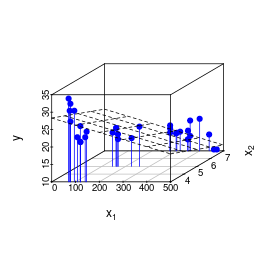
\includegraphics[width=0.9\textwidth, trim=0 40 0 0, clip]{
    figure/lm_3d.png} \\
    \tiny{Linear regression hyperplane}
  \end{center}
\end{minipage}
\begin{minipage}[b]{0.32\textwidth}
  \begin{center}
    % 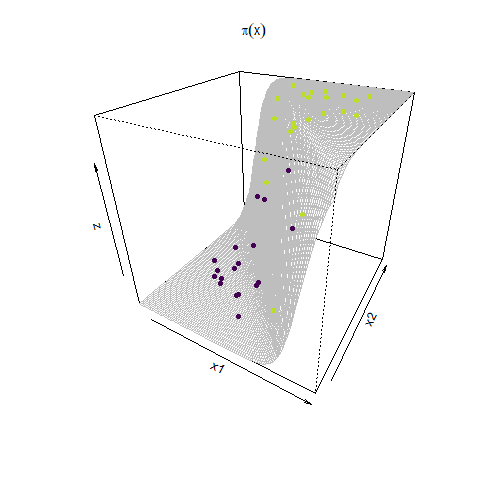
\includegraphics[width=0.7\textwidth, trim=0 40 0 0, clip]{
    % ../slides/supervised-classification/figure_man/logreg-2vars-surface}\\
    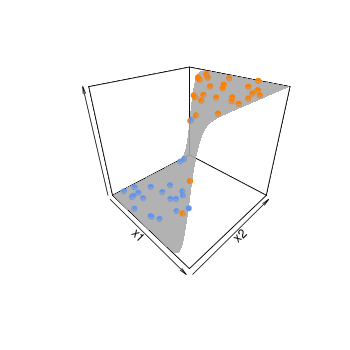
\includegraphics[width=0.7\textwidth, trim=30 50 0 0, clip]{figure/logreg_3d}\\
    \tiny{Logistic function for bivariate input and loss-minimal $\thetab$}
  \end{center}
\end{minipage}
\begin{minipage}[b]{0.32\textwidth}
  \begin{center}
    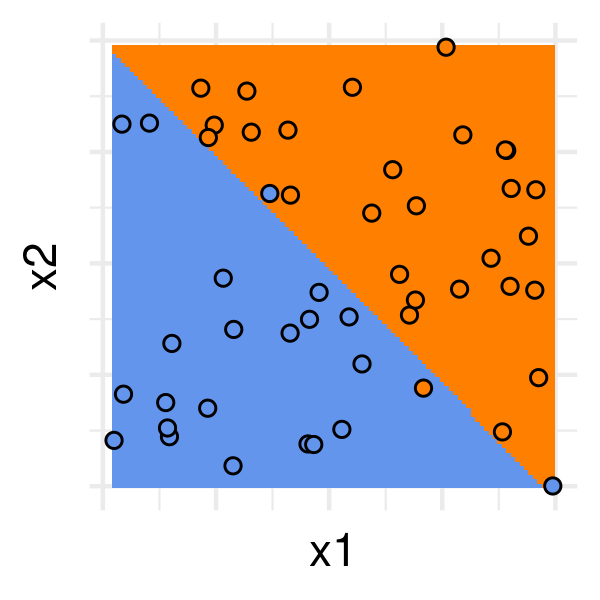
\includegraphics[width=0.5\textwidth]{figure/logreg_2d}\\
    % 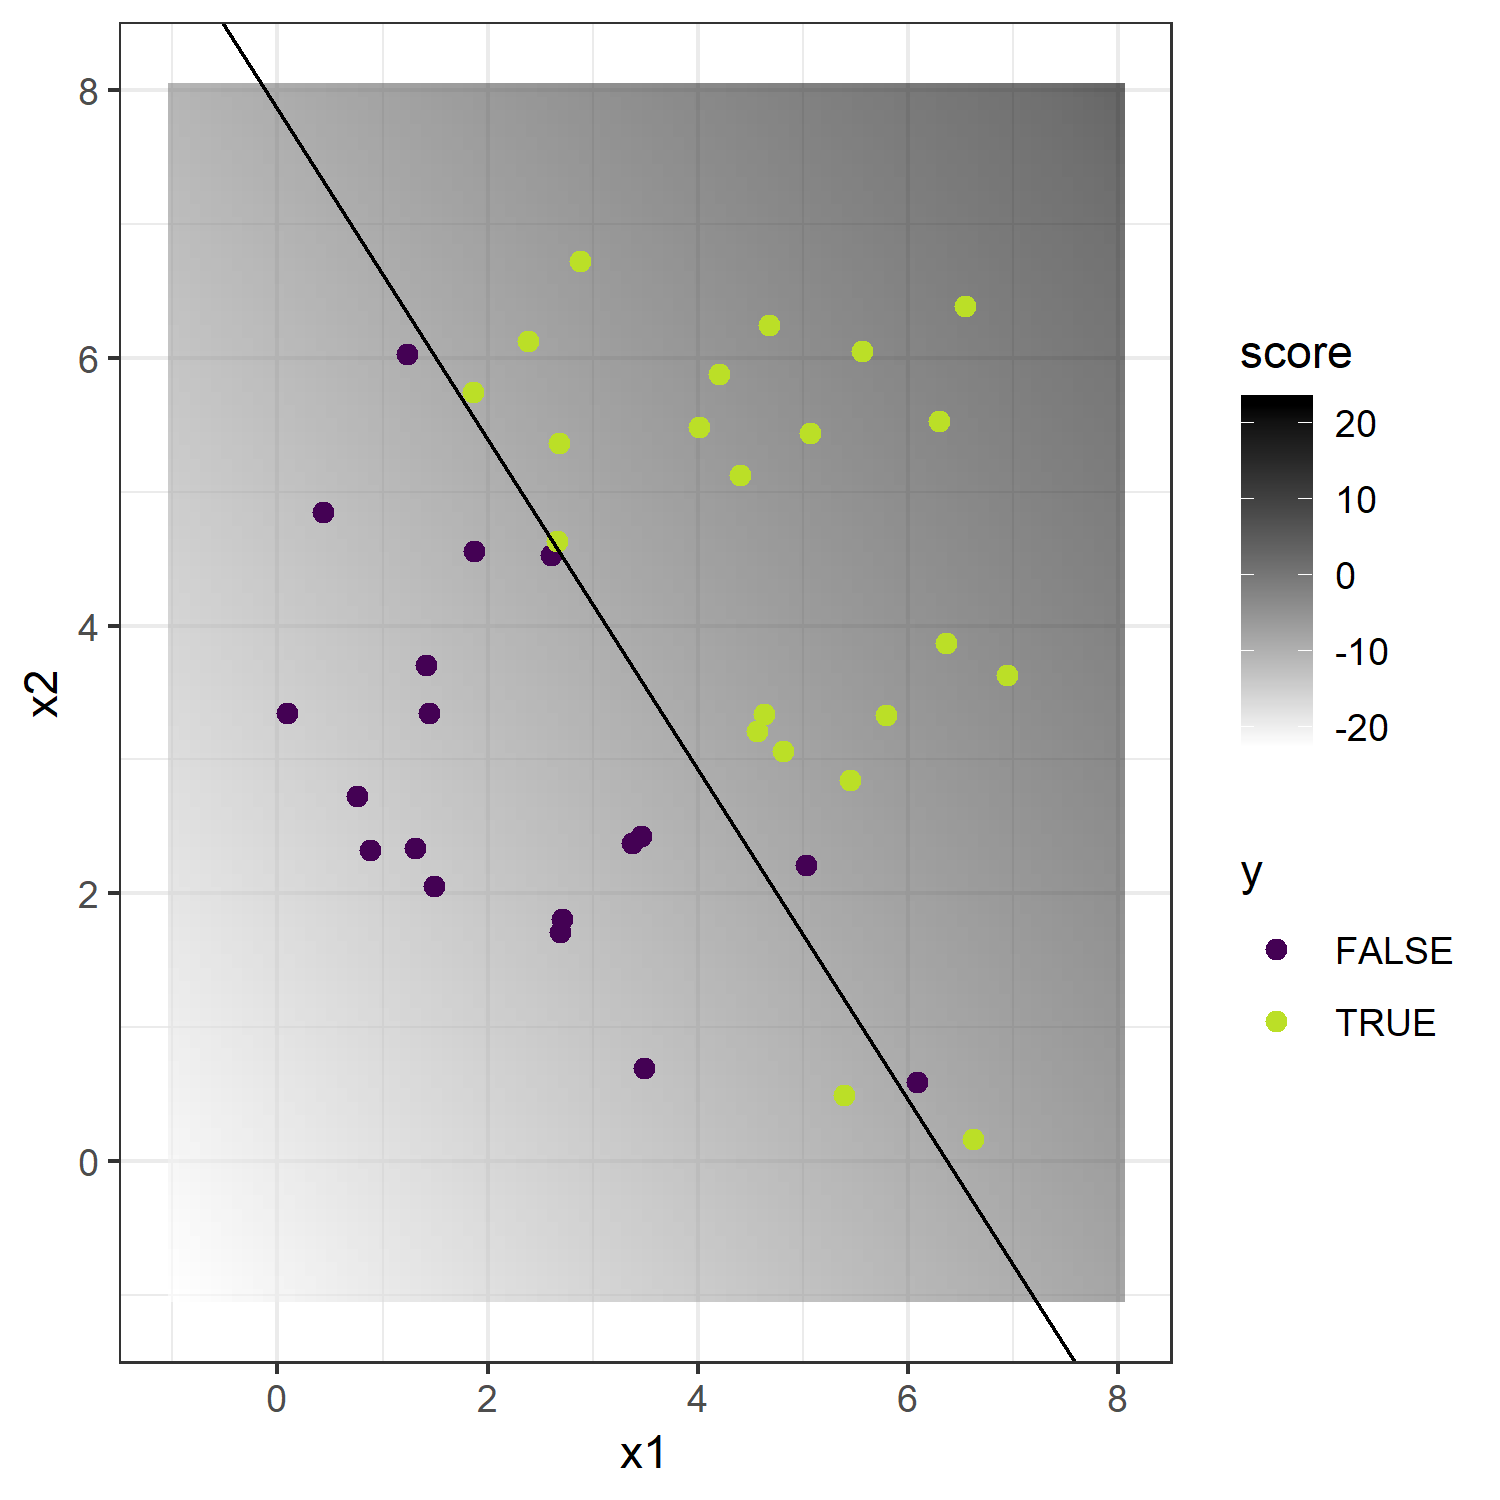
\includegraphics[width=0.6\textwidth]{
    % ../slides/supervised-classification/figure_man/logreg-2vars-data} \\
    \tiny{Corresponding separating hyperplane}
\end{center}
\end{minipage}

\framebreak

\highlight{Empirical risk}

\begin{itemize}
  \item \textbf{Linear regression}
  \begin{itemize}
    
    \item Typically, based on \textbf{quadratic} loss: $\risket = 
    \sumin \left(\yi - \fxit \right)^2$ \\
    $\Rightarrow$ corresponding to ordinary-least-squares (OLS) estimation
    \item Alternatives: e.g., \textbf{absolute} or \textbf{Huber} loss (both 
    improving robustness)
  \end{itemize}
  \item \textbf{Logistic regression:} based on 
  \textbf{Bernoulli/log/cross-entropy} loss ~ 
  $\Rightarrow \risket = \sumin -\yi \log 
  \left(\pixii\right) - (1 - \yi) \log \left(1 - \pixii \right)$
\end{itemize}

\medskip

\highlight{Optimization}
\begin{itemize}
  \item For \textbf{OLS}: analytically with 
  $\thetabh = \olsest$ ~~
  ($\Xmat \in \R^{n \times p}$ : matrix of feature vectors)
  \item For \textbf{other loss functions}: numerical optimization 
\end{itemize}

\medskip

\highlight{Hyperparameters} ~~ None

\medskip

% \highlight{Runtime behavior} ~~ $\mathcal{O}(p^2 \cdot n + p^3)$ for $n$ 
% observations and $p$ features

\end{vbframe}

% ------------------------------------------------------------------------------

\begin{frame}{Linear Models -- Pro's \& Con's}



\begin{columns}[onlytextwidth]
  \begin{column}{0.5\textwidth}
    \highlight{Advantages}
    
    \begin{itemize}
      \positem \textbf{Simple and fast} implementation
      \positem \textbf{Analytical} solution for quadratic loss
      \positem \textbf{Cheap} computation
      \positem Applicable for any \textbf{dataset size}, as long as number of 
      observations $\gg$ number of features
      \positem Flexibility \textbf{beyond linearity} with polynomials, 
      trigonometric transformations etc.
      \positem Intuitive \textbf{interpretability} via feature effects
      % \positem fits \textbf{linearly} separable data sets very well
      \positem Statistical hypothesis \textbf{tests} for effects available

    \end{itemize}
  \end{column}

  \begin{column}{0.5\textwidth}
    \highlight{Disadvantages}
    
    \begin{itemize}
      \negitem \textbf{Nonlinearity} of many real-world problems
      \negitem Further restrictive \textbf{assumptions}: linearly independent 
      features, homoskedastic residuals, normality of conditional response
      \negitem \textbf{Sensitivity} w.r.t. outliers and noisy data (especially 
      with L2 loss)
      \negitem Risk of \textbf{overfitting} in higher dimensions
      \negitem Feature \textbf{interactions} must be handcrafted, so higher
      orders practically infeasible
      \negitem No handling of \textbf{missing} data
    \end{itemize}
  \end{column}
\end{columns}

\vfill

\small

\conclbox{Simple, highly interpretable method, but 
with strong assumptions, practical limitations, and risk of overfitting}

\end{frame}

% ------------------------------------------------------------------------------

\begin{frame}{Linear Models -- regularization}

\highlight{Idea}

\begin{itemize}
  \item Unregularized LM: risk of \textbf{overfitting} in high-dimensional 
  space with only few observations
  \item \textbf{Goal}: find compromise between model fit and generalization by 
  adding \textbf{penalty term}
\end{itemize}

\medskip

% \highlight{Hypothesis space} ~~\\
% $\Hspace = \left\{f: \Xspace \to \R ~|~\fx = \phi(\thetab^\top \xv)\right\}$, 
% where $\phi(\cdot)$ is a transformation function.


%$\Hspace = \{ \theta_0 + \thx\ |\ (\theta_0, \thetab) \in \R^{p+1} \} $

\medskip

\highlight{Regularized empirical risk}

\begin{itemize}
  \item Empirical risk function \textbf{plus complexity penalty} 
  $J(\thetab)$, controlled by shrinkage parameter $\lambda > 0$: \\
  $\riskrt := \risket + \lambda \cdot J(\thetab).$ 
  \item Popular regularizers
  \begin{itemize} 
    \item \textbf{Ridge} regression: L2 penalty $J(\thetab) = \|\thetab\|_2^2 $
    \item \textbf{LASSO} regression: L1 penalty $J(\thetab) = \|\thetab\|_1 $
  \end{itemize}
\end{itemize}

\medskip

\highlight{Optimization under regularization}
\begin{itemize}
  \item \textbf{Ridge}: analytically with 
  $\thetabh_{\text{Ridge}} = (\Xmat^\top \Xmat  + \lambda \id)^{-1} \Xmat^\top 
  \yv$
  \item \textbf{LASSO}: numerically with, e.g., (sub-)gradient descent
\end{itemize}

\end{frame}

% ------------------------------------------------------------------------------

\begin{frame}{Linear Models -- regularization}

\highlight{Choice of regularization parameter}

\begin{itemize}
  \item Standard hyperparameter optimization problem
  \item E.g., choose $\lambda$ with minimum mean cross-validated error 
  (default in R package \texttt{glmnet})
\end{itemize}

\medskip

\highlight{Ridge vs. LASSO} 

\begin{itemize}
  \item \textbf{Ridge}
  \begin{itemize} 
    \item Overall smaller, but still dense $\thetab$
    \item Applicable with large number of influential features, handling 
    correlated variables by shrinking their coefficients to equal degree
  \end{itemize}
  \item \textbf{LASSO}
  \begin{itemize} 
    \item Actual variable selection
    \item Suitable for sparse problems, ineffective with correlated 
    features (randomly selecting one)
  \end{itemize}  
  \item Neither overall better $\rightarrow$ compromise: \textbf{elastic net}
  = weighted 
  combination of Ridge and LASSO
\end{itemize}


\end{frame}

% ------------------------------------------------------------------------------

\begin{frame}{Linear Models -- Practical hints}

\highlight{Implementation}

\begin{itemize}
  \item \textbf{R:}
  \begin{itemize}
    \item \textbf{Unregularized:} \texttt{mlr3} learner \texttt{LearnerRegrLM}, 
    calling \texttt{stats::lm()} / \texttt{mlr3} learner 
    \texttt{LearnerClassifLogReg}, calling \texttt{stats::glm()}
    \item \textbf{Regularized:} \texttt{mlr3} learners 
    \texttt{LearnerClassifGlmnet} / 
    \texttt{LearnerRegrGlmnet}, calling \texttt{glmnet::glmnet()}
  \end{itemize}
  \item \textbf{Python:} \texttt{LinearRegression} from package 
  \texttt{sklearn.linear\_model}, package for advanced statistical parameters 
  \texttt{statsmodels.api} 
\end{itemize}

%% WOULD DELTETE THIS!
%  \highlight{\textcolor{blue}{Check assumptions??} }\\
% Linear models are effective if the following assumptions are fulfilled:
%  \begin{itemize}
%   \item \textbf{linearity}: The expected response is a linear combination of the features.
%   \item \textbf{homoscedasticity}: The variance of residuals is equal for all features.
%   \item \textbf{independence}: All observations are independent of each other.
%   \item \textbf{normality}: Y is normally distributed for any fixed value of the features
% \end{itemize}

\end{frame}

% \section{Regularized Linear Models}
% \begin{frame}{Regularized LM -- method summary}

\highlight{General idea}

\begin{itemize}
  \item Unregularized LM: risk of \textbf{overfitting} in high-dimensional 
  space with only few observations
  \item \textbf{Goal}: find compromise between model fit and generalization
\end{itemize}

\medskip

% \highlight{Hypothesis space} ~~\\
% $\Hspace = \left\{f: \Xspace \to \R ~|~\fx = \phi(\thetab^\top \xv)\right\}$, 
% where $\phi(\cdot)$ is a transformation function.


%$\Hspace = \{ \theta_0 + \thx\ |\ (\theta_0, \thetab) \in \R^{p+1} \} $

\medskip

\highlight{Empirical risk}

\begin{itemize}
  \item Empirical risk function \textbf{plus complexity penalty} 
  $J(\thetab)$, controlled by shrinkage parameter $\lambda > 0$: \\
  $\riskrt := \risket + \lambda \cdot J(\thetab).$ 
  \item Popular regularizers
  \begin{itemize} 
    \item \textbf{Ridge} regression: L2 penalty $J(\thetab) = \|\thetab\|_2^2 $
    \item \textbf{LASSO} regression: L1 penalty $J(\thetab) = \|\thetab\|_1 $
  \end{itemize}
\end{itemize}

\medskip

\highlight{Optimization}
\begin{itemize}
  \item \textbf{Ridge}: analytically with 
  $\thetabh_{\text{Ridge}} = (\Xmat^\top \Xmat  + \lambda \id)^{-1} \Xmat^\top 
  \yv$
  \item \textbf{LASSO}: numerically with, e.g., (sub-)gradient descent
\end{itemize}

\medskip

\highlight{Hyperparameters} ~~ Shrinkage parameter $\lambda$

\medskip

% \highlight{Runtime behavior} ~~ $\mathcal{O}(p^2 \cdot n + p^3)$ for $n$ 
% observations and $p$ features 

\end{frame}

% ------------------------------------------------------------------------------

\begin{frame}{Regularized LM -- Practical hints}

\highlight{Choice of regularization parameter}

\begin{itemize}
  \item Standard hyperparameter optimization problem
  \item E.g., choose $\lambda$ with minimum mean cross-validated error 
  (default in R package \texttt{glmnet})
\end{itemize}

\medskip

\highlight{Ridge vs. LASSO} 

\begin{itemize}
  \item \textbf{Ridge}
  \begin{itemize} 
    \item Overall smaller, but still dense $\thetab$
    \item Suitable with many influential features present, handling correlated 
    features by shrinking their coefficients equally
  \end{itemize}
  \item \textbf{LASSO}
  \begin{itemize} 
    \item Actual variable selection
    \item Suitable for sparse problems, ineffective with correlated 
    features (randomly selecting one)
  \end{itemize}  
  \item Neither overall better -- compromise: \textbf{elastic net} \\
  $\rightarrow$ weighted 
  combination of Ridge and LASSO regularizers
\end{itemize}

\medskip

\highlight{Implementation}

\begin{itemize}
    \item \textbf{R:} \texttt{mlr3} learners \texttt{LearnerClassifGlmnet} / 
    \texttt{LearnerRegrGlmnet}, calling \texttt{glmnet::glmnet()}
    \item \textbf{Python:} \texttt{LinearRegression} from package 
    \texttt{sklearn.linear\_model}, package for advanced statistical parameters 
    \texttt{statsmodels.api} 
  \end{itemize}

\end{frame}


\section{Generalized Additive Models (GAM)}
\begin{vbframe}{Generalized Additive Models -- method summary}

% \maketag{SUPERVISED} 
\maketag{regression} \maketag{classification} \maketag[50]{(NON)PARAMETRIC}
\maketag[50]{WHITE-BOX} \maketag[50]{Feature selection}
\medskip

\highlight{General idea}
\begin{itemize}
  \item Same as GLM, but introduce \textbf{flexibility} through
  \textbf{nonlinear (smooth)} effects $f_j(x_j)$
  \item Typically, combination of linear \& smooth effects
  \item Smooth effects also conceivable for feature interactions
\end{itemize}
\medskip

\highlight{Hypothesis space} ~~
$\Hspace = \left\{f: \Xspace \to \R ~|~\fx = \phi \left(\theta_0 + \sumjp
f_j(x_j) \right) \right\}$,
with suitable transformation $\phi(\cdot)$, intercept term $\theta_0$, and smooth
functions $f_j(\cdot)$

\vfill

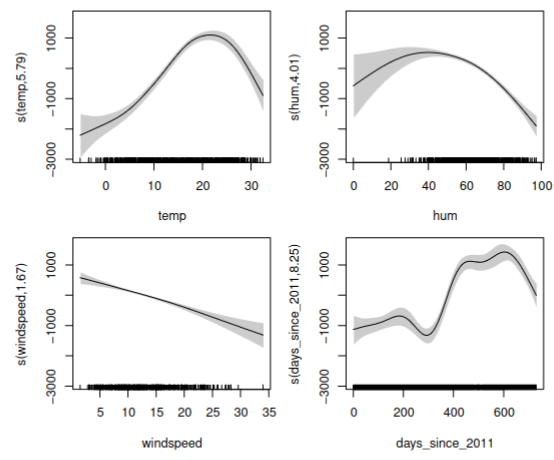
\includegraphics[width=0.2\textwidth]{figure/smooth_effects}
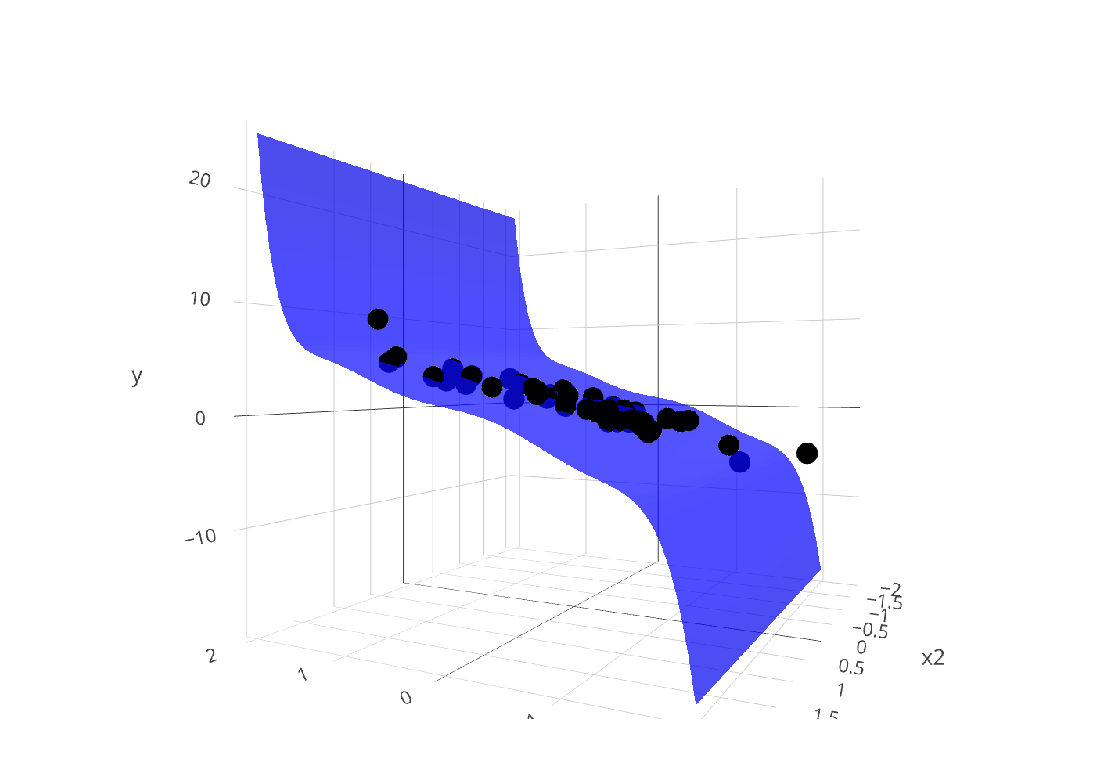
\includegraphics[width=0.2\textwidth]{figure/reg_poly_biv}
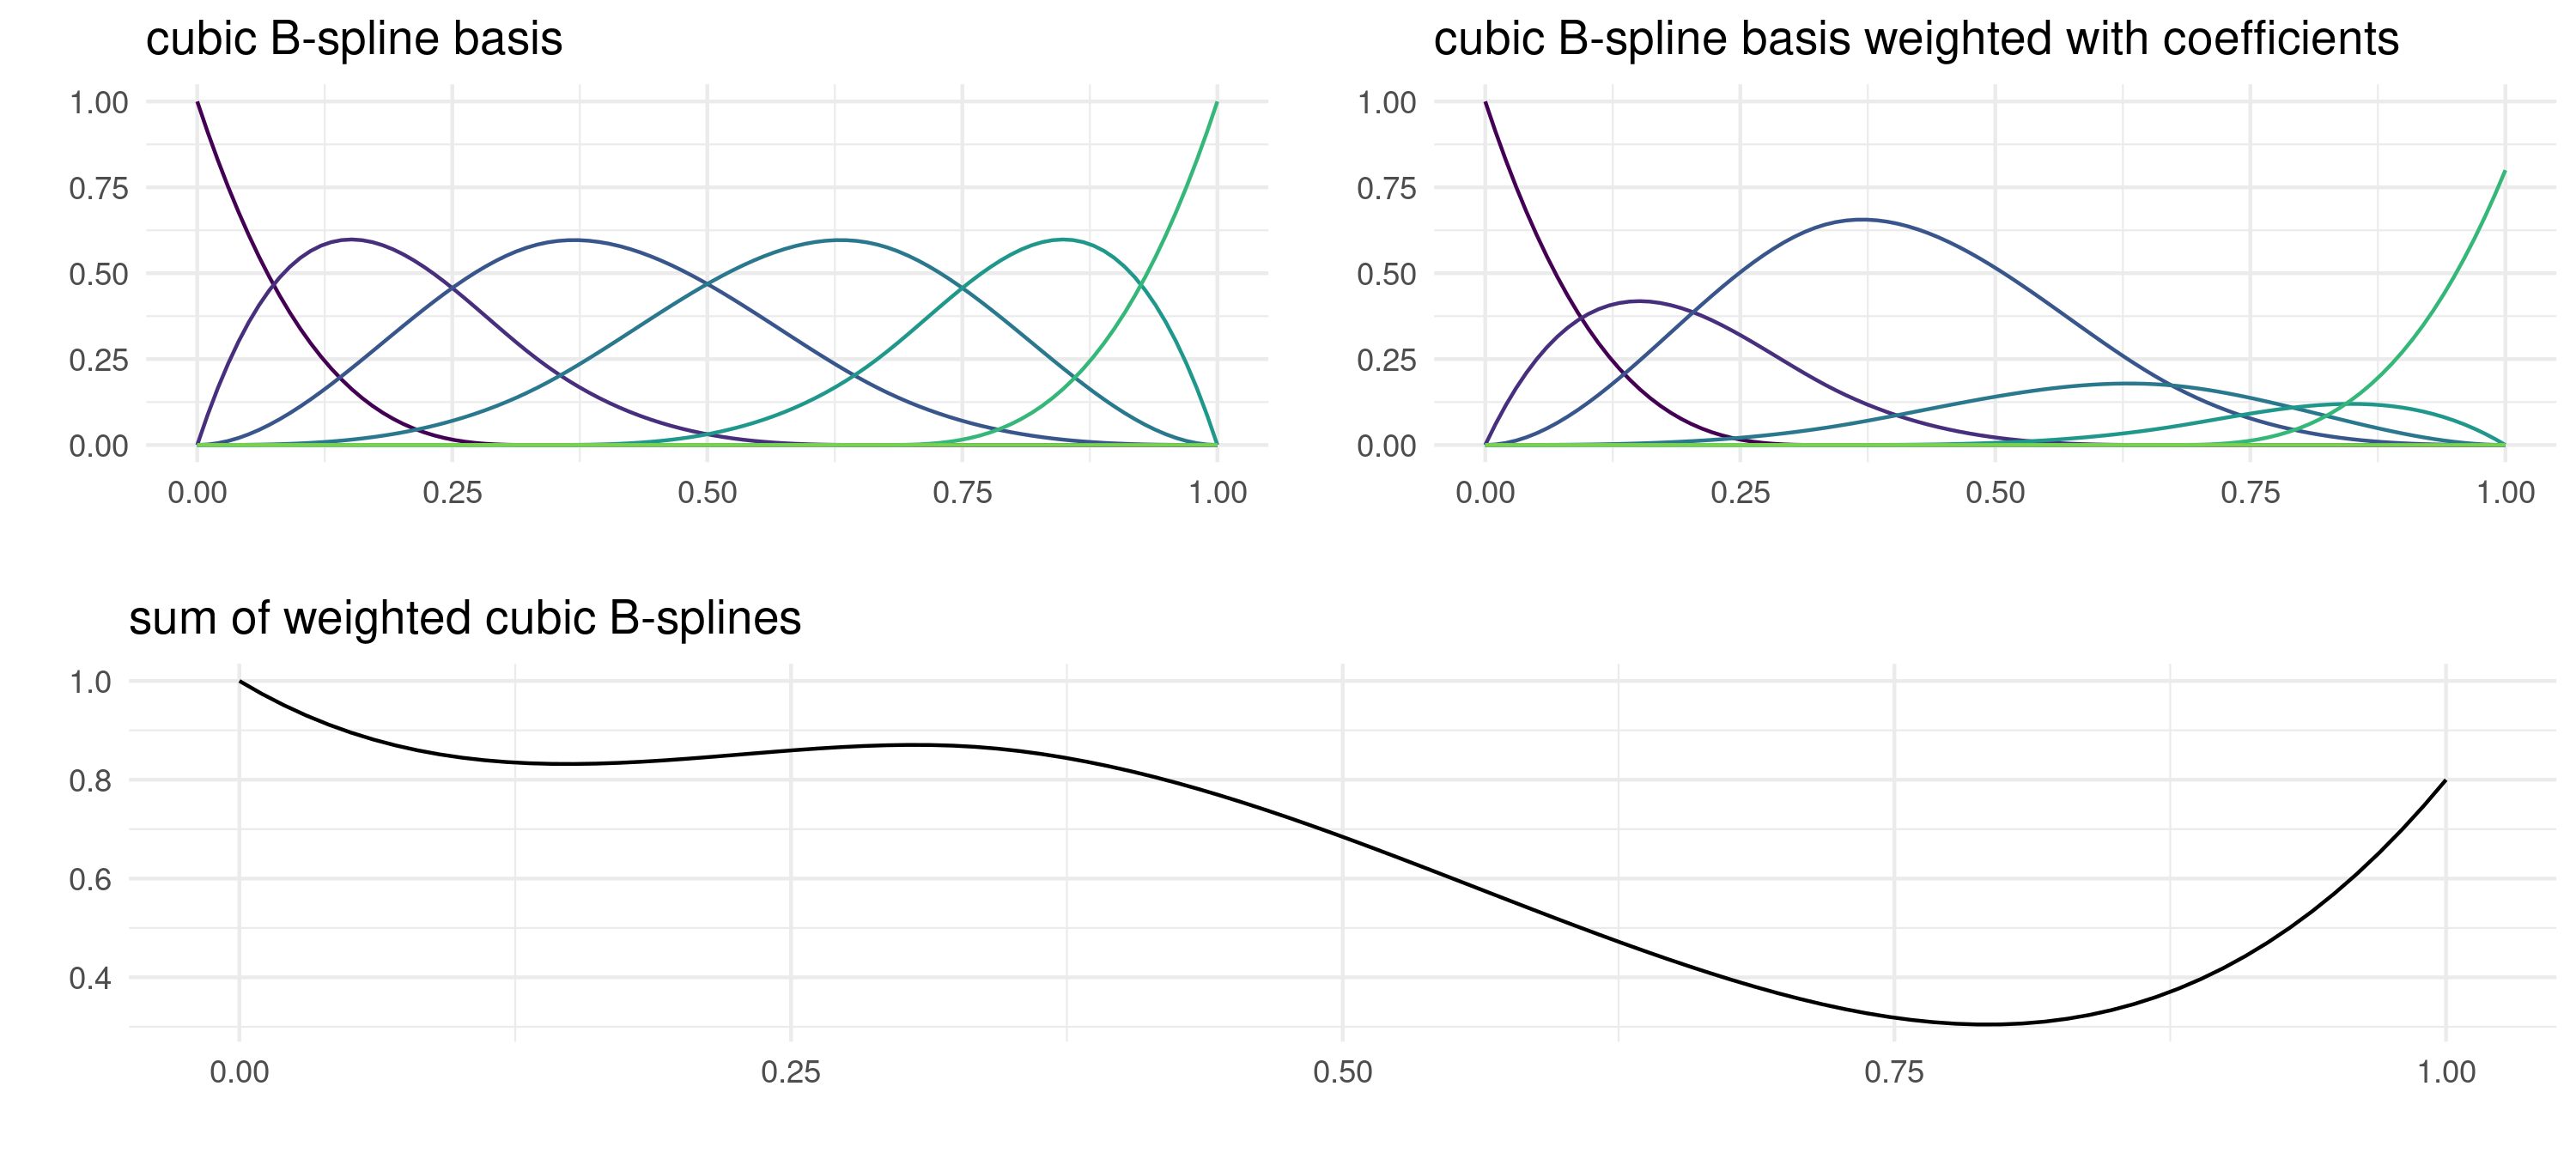
\includegraphics[width=0.4\textwidth]{figure/bspline-basis}

\textcolor{blue}{Figures still placeholders}

\framebreak

\highlight{Smooth functions}

\begin{itemize}
  \item Nonparametric/semiparametric/parametric approaches conceivable
  \item Frequently: express $f_j$ as weighted sum of \textbf{basis functions}
  $\rightsquigarrow$ model \textbf{linear} in weight coefficients again
  \begin{itemize}
      \item Use fixed basis of functions $b_1, \dots, b_K$ and estimate
      associated coefficients $\gamma_1, \dots, \gamma_K$ \\ $\rightsquigarrow$
      $f_j(x_j) = \sum_{k=1}^{K_j} \gamma_{j, k} b_k(x_j)$
      \item Popular types of basis functions
      \begin{itemize}
        \footnotesize
        \item Polynomial $\rightsquigarrow$ smoothing/TP-/B-\textbf{splines}
        \item Radial $\rightsquigarrow$ \textbf{Kriging}
        \item Trigonometric $\rightsquigarrow$ \textbf{Fourier/wavelet} forms
      \end{itemize}
    \end{itemize}
    \item Alternatives: \textbf{local regression (LOESS)}, other
    kernel-smoothing approaches, \dots
\end{itemize}

\medskip

\highlight{Regularization}
\begin{itemize}
    \item Smooth functions possibly very flexible $\rightsquigarrow$
    regularization vital to prevent overfitting
    \item Control \textbf{smoothness}
    \begin{itemize}
      \item \textbf{Basis-function approaches}: impose penalty on coefficients
      (e.g., magnitude or differences between coefficients of neighboring
      components) \& control associated hyperparameter
      \item \textbf{Local smoothers}: control width of smoothing window
      (larger $\rightsquigarrow$ smoother)
    \end{itemize}
\end{itemize}

\end{vbframe}

% ------------------------------------------------------------------------------

\begin{frame}{Generalized Additive Models -- implementation}

\highlight{Loss functions} ~~ Same as in GLM $\rightsquigarrow$ essentially:
use \textbf{negative log-likelihood}

\medskip

\highlight{Optimization}
\begin{itemize}
  \item \textbf{Coefficients} (of smooth + linear terms):
  penalized MLE, Bayesian inference
  \item \textbf{Smoothing hyperparameters}: typically, generalized
  cross-validation
\end{itemize}

\medskip

\highlight{Implementation}

\begin{itemize}
  \item \textbf{R:} \texttt{mlr3} learner \texttt{LearnerRegrGam},
    calling \texttt{mgcv::gam()}
  \begin{itemize}
      \item Smooth terms: \texttt{s(\dots, bs="<basis>")} or \texttt{te(\dots)}
      for multivariate (tensorproduct) effects
      \item Link functions: \texttt{family=$\{$Gamma, Binomial, \dots $\}$}
  \end{itemize}
    \item \textbf{Python}: \texttt{GLMGam} from package \texttt{statsmodels};
    package \texttt{pygam}
\end{itemize}

\medskip
\begin{columns}[onlytextwidth]
  \begin{column}{0.5\textwidth}
    \highlight{Advantages}

    Strengths of GLMs, plus \dots
    \begin{itemize}
      \positem Much \textbf{higher flexibility} via smooth effects
      \positem Easy to \textbf{combine} linear \& nonlinear effects
    \end{itemize}
  \end{column}

  \begin{column}{0.5\textwidth}
    \highlight{Disadvantages}

    Shortcomings of GLMs, plus \dots
    \begin{itemize}
      \negitem Harder to \textbf{optimize}
      \negitem Not quite as easy to \textbf{interpret}
      \negitem Prone to \textbf{overfitting}
      \negitem Additional \textbf{hyperparameters} (type of smooth functions,
      smoothness degree, \dots)
    \end{itemize}
  \end{column}
\end{columns}

\end{frame}


\section{Classification \& Regression Trees (CART)}
\begin{frame}{CART -- method summary}

\footnotesize

% \maketag{Supervised} 
\maketag{regression} \maketag{classification}
\maketag{Nonparametric} \maketag{White-box} \maketag{Feature selection}

\medskip

\begin{columns}[T, totalwidth=\textwidth]
\begin{column}{0.6\textwidth}
\highlight{General idea}
\begin{itemize}
  \item Start at root node containing all data
  \item Perform repeated \textbf{binary splits} in feature space to obtain
  \textbf{rectangular partitions} at terminal nodes $Q_1, \dots, Q_M$
  \item Splits based on reduction of node \textbf{impurity} \\
  $\rightarrow$ empirical risk minimization (\textbf{ERM})
  \item In each step:
  \begin{itemize}
    \item Find \textbf{optimal split} (feature-threshold combination) \\
    $\rightarrow$ greedy search
    \item Assign constant prediction $c_m$ to all obs. in region $Q_m$\\
    $\rightarrow$ Regression: $c_m$ is average of $y$ \\
    $\rightarrow$ Classif.: $c_m$ is majority class (or class proportions)
    
  \item Stop when a pre-defined criterion is reached\\
  $\rightarrow$ See \highlight{Complexity control}
  \end{itemize}
  % \item Unless interrupted, splitting continues until each observation ends up 
  % in its own leaf node $\rightarrow$ \textbf{control complexity}
\end{itemize}

\medskip

%\medskip
    \highlight{Hypothesis space} ~~
$\Hspace = \left\{ \fx: \fx = \sum\limits_{m = 1}^M c_m \I(\xv \in Q_m) 
\right\}$

\end{column}
\begin{column}{0.45\textwidth}
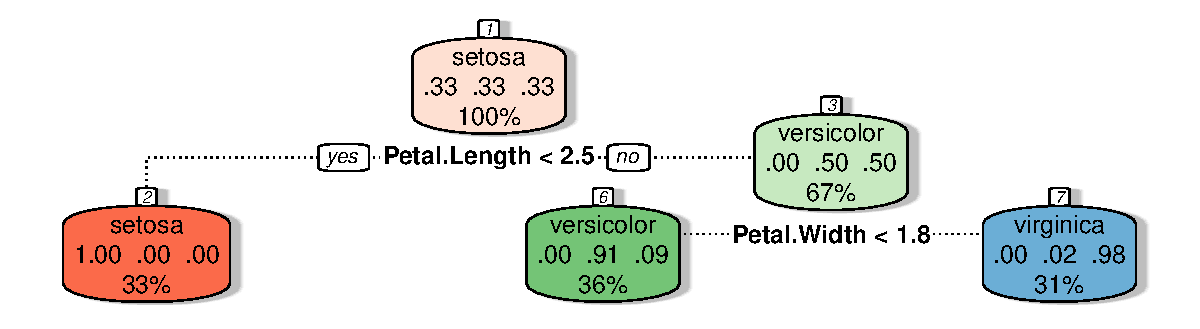
\includegraphics[width=\textwidth]{../slides/trees/figure/cart_treegrow_22}
\includegraphics[width=\textwidth]{   ../slides/trees/figure/cart_splitcriteria_1} 
\end{column}
\end{columns}


% \begin{minipage}[b]{0.5\textwidth}
%   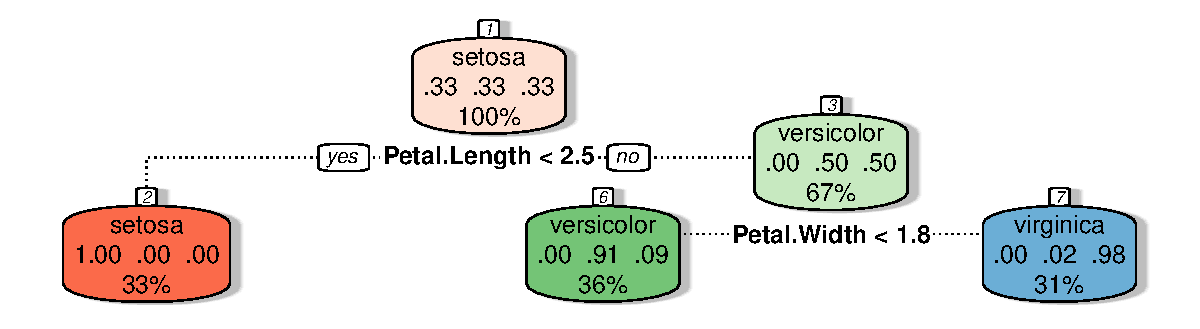
\includegraphics[width=\textwidth]{../slides/trees/figure/cart_treegrow_22} \\
%   \tiny{Classification tree for \texttt{iris} data after 3 splits}
% \end{minipage}
% \begin{minipage}[b]{0.49\textwidth}
%   \centering
%   \includegraphics[width=0.9\textwidth]{
%   ../slides/trees/figure/cart_splitcriteria_1} \\
%   \tiny{Corresponding prediction surface with axis-aligned boundaries}
% \end{minipage}%

\end{frame}

% ------------------------------------------------------------------------------

\begin{frame}{CART -- method summary}

\footnotesize

\begin{columns}[T, totalwidth=\linewidth]
    \begin{column}{0.6\linewidth}
    
\highlight{Empirical risk} \\
    \begin{itemize}
\item Splitting \textbf{feature $x_j$ at split point $t$} divides a parent node $\Np$ into two child nodes:
 \begin{align*}\Nl = \{ (\xv, y) \in \Np: x_j \leq t \} \text{ and } \Nr = \{ (\xv, y) \in \Np: x_j > t \}
      \end{align*}
  %\item Calculated after each split, i.e., at each node $\Np_t$ (which is not necessarily the terminal node $Q_t$)
  
\end{itemize}
    \end{column}
    \begin{column}{0.4\linewidth}
{\centering 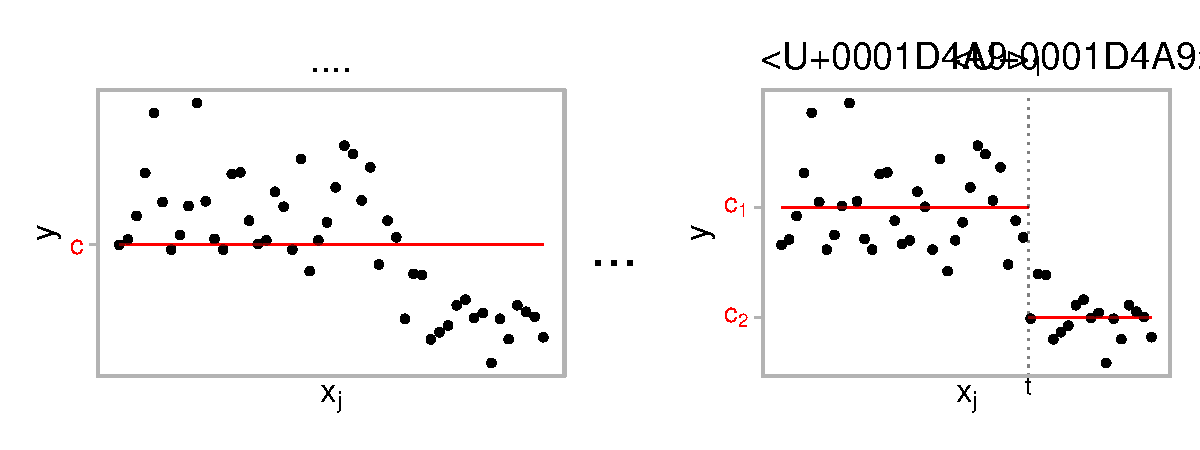
\includegraphics[width=0.975\textwidth]{../slides/trees/figure/cart_splitcriteria_2.pdf} 
}
\end{column}
\end{columns}
\begin{itemize}
  \item Compute empirical risks in child nodes and minimize their sum to find best split (impurity reduction):
     \begin{align*}
      \argmin_{j, t} \risk(\Np, j, t) &= \argmin_{j, t} \tfrac{|\Nl|}{|\Np|} \risk(\Nl) + \tfrac{|\Nr|}{|\Np|} \risk(\Nr)
      \end{align*}
      
  \item In general, compatible with arbitrary losses -- typical choices:
  \begin{itemize}
    \footnotesize
    %\item $g$-way classification:
    %\begin{itemize}
      %\footnotesize
    %   \item $g$-way classification (\textbf{Brier score}): ~~
    %   $\risk(\Np) = \sum\limits_{(\xv,y) \in \Np} \sumkg
    %   \hat{\pik}^{(\Np)} (1 - \hat{\pik}^{(\Np)} )$
    %   % $\risk(\Np) = \sum\limits_{(\xv,y) \in \Np} \sumkg \left( \I(y = k)
    %   % - \pikx \right)^2$ 
    %   $\rightarrow$ \textbf{Gini} impurity
    %   \item $g$-way classification (\textbf{Bernoulli} loss): ~~
    %   $\risk(\Np) = \sum\limits_{(\xv,y) \in \Np} - \sumkg
    %   \hat{\pik}^{(\Np)} \log \hat{\pik}^{(\Np)}$
    %   % $\risk(\Np) = \sum\limits_{(\xv,y) \in \Np} \sumkg \I(y = k) \cdot
    %   % \log(\pikx)$ 
    %   $\rightarrow$ \textbf{entropy} impurity
    % %\end{itemize}

      \item $g$-way classification:
      \begin{tabular}{c |@{\vline}| c} 
 \textbf{Brier score} $\rightarrow$ \textbf{Gini} impurity & \textbf{Bernoulli} loss $\rightarrow$ \textbf{entropy} impurity \\ 
 \hline\\[-2ex]
 $\risk(\Np) = \sum_{(\xv,y) \in \Np} \sum_{k=1}^g
      \hat{\pik}^{(\Np)} (1 - \hat{\pik}^{(\Np)} )$ & $\risk(\Np) = \sum_{(\xv,y) \in \Np} - \sum_{k=1}^g
      \hat{\pik}^{(\Np)} \log \hat{\pik}^{(\Np)}$
\end{tabular}
      
    \item Regression (\textbf{quadratic} loss): ~~
    $\risk(\Np_t) = \sum_{(\xv,y) \in \Np} (y - c)^2$ with $c = \frac{1}{|\Np|} \sum_{(\xv,y) \in \Np} y$
  \end{itemize}
\end{itemize}

\medskip

\highlight{Optimization}

\begin{itemize}
  \item \textbf{Exhaustive} search over all split candidates, choice of 
  risk-minimal split
  \item In practice: reduce number of split candidates (e.g., using quantiles instead of all observed values)
\end{itemize}

\medskip

\highlight{Hyperparameters} ~~ \textbf{Complexity}, i.e., 
number of terminal nodes $T$ (controlled indirectly, see \highlight{Implementation}) 

\end{frame}

% ------------------------------------------------------------------------------

\begin{frame}{CART -- Pro's \& Con's}

\begin{columns}[onlytextwidth]
  \begin{column}{0.5\textwidth}
    \highlight{Advantages}
    \footnotesize
    \begin{itemize}
      \positem \textbf{Easy} to understand \& visualize (\textbf{interpretable})
      \positem Built-in \textbf{feature selection}\\
      $\rightarrow$ e.g., when features are not used for splitting
      \positem Applicable to \textbf{categorical} features \\
      $\rightarrow$ e.g., $2^m$ possible binary splits for $m$ categories\\
       $\rightarrow$ for regr. with L2-loss and binary classif., categories can be sorted $\Rightarrow$ $m-1$ binary splits 
      \positem Handling of \textbf{missings} possible via surrogate splits
      \positem \textbf{Interaction} effects between features naturally included, 
      even of higher order
      \positem \textbf{Fast} computation and good scalability
      \positem High \textbf{flexibility} (custom split criteria or leaf-node 
      prediction rules)   
    \end{itemize}
  \end{column}
  \begin{column}{0.5\textwidth}
    \highlight{Disadvantages}
    \footnotesize
    \begin{itemize}
      \negitem Rather \textbf{poor generalization} when used stand-alone 
      \negitem High \textbf{variance/instability}: model can change a lot when training data is minimally changed
      \negitem Risk of \textbf{overfitting} if tree are grown too deep
      \negitem Not well-suited to model \textbf{linear} relationships
      \negitem \textbf{Bias} toward features with many categories
    \end{itemize}
  \end{column}
\end{columns}

\vfill

\small

\conclbox{Simple, good with feature selection and highly interpretable, but not 
the most performant learner}

\end{frame}

% ------------------------------------------------------------------------------

\begin{frame}{CART -- Practical hints}

\footnotesize

\highlight{Hyperparameters and complexity control}

\begin{itemize}
  \item Unless interrupted, splitting continues until we have pure leaf nodes (costly + overfitting)
  \item Hyperparameters: Complexity controlled via tree depth, minimum number of observations per node, maximum number of leaves, minimum risk reduction per split, ...
  \item Limit tree growth / complexity via
  \begin{itemize}
    \item \textbf{Early stopping:} stop growth prematurely \\ $\rightarrow$ hard 
    to determine good stopping point before actually trying all combinations
    \item \textbf{Pruning:} grow deep trees and cut back in risk-optimal manner afterwards
  \end{itemize}
\end{itemize}

\medskip

\highlight{Bagging / boosting} ~~ 
As CART is a highly \textbf{unstable} learner, it is used as base learner in bagging (random forest) or boosting ensembles.

\medskip

\highlight{Some other decision trees}
\begin{columns}[T, totalwidth=\linewidth]
    \begin{column}{0.39\linewidth}
    \vspace{-\parsep}
        \begin{itemize}
%\item AID (Sonquist and Morgan, 1964)
\item CHAID (Kass, 1980)%\\
%$\rightarrow$ Multi-level splits
\item C4.5 (Quinlan, 1993)
\end{itemize}
    \end{column}
    \begin{column}{0.59\linewidth}
    \vspace{-\parsep}
        \begin{itemize}
\item Linear Model Trees (Potts, 2004)
\item Unbiased Recursive Partitioning (Hothorn et al., 2006)
\end{itemize}
    \end{column}
\end{columns}
   
\medskip

\highlight{Implementation}
\begin{itemize}
  \item \textbf{R:} \texttt{mlr3} learners \texttt{LearnerClassifRpart} / 
    \texttt{LearnerRegrRpart}, calling \texttt{rpart::rpart()}
  \item \textbf{Python:} \texttt{DecisionTreeClassifier} / 
  \texttt{DecisionTreeRegressor} from package \texttt{scikit-learn}
\end{itemize}

\end{frame}


\section{Random Forests}
\begin{frame}{Random Forests -- method summary}

% \maketag{SUPERVISED} 
\maketag{regression} \maketag{classification}
\maketag{NONPARAMETRIC} \maketag[50]{BLACK-BOX} \maketag{FEATURE SELECTION}

\medskip

\highlight{General idea} 
\begin{itemize}
  \item \textbf{Bagging ensemble} of $M$ tree \textbf{base learners} fitted on \textbf{bootstrap} data samples
   \begin{itemize}
    \item Use unstable, \textbf{high-variance} base learners ~~$\Rightarrow$
    let trees grow to full size
    \item Mitigate individual trees' bias by promoting \textbf{decorrelation} 
    ~~ $\Rightarrow$ use random subset of 
    candidate features for each split
  \end{itemize}
  \item \textbf{Predict} via averaging (regression) or majority vote 
  (classification) of base learners
\end{itemize}

\medskip

\highlight{Hypothesis space} ~~
$\Hspace = \left\{ \fx: \fx = \frac{1}{M} \sum\limits_{m = 1}^M 
\sum\limits_{t = 1}^{T^{[m]}} 
c_t^{[m]} \I(\xv \in Q_t^{[m]}) \right\}$

\medskip

\begin{minipage}[b]{0.65\textwidth}
  % FIGURE SOURCE: https://docs.google.com/presentation/d/1xodP6ayu1Gay6mMKgzVWYEFmSoeG5kNuqsaTkFFmd78  /edit
  \centering
  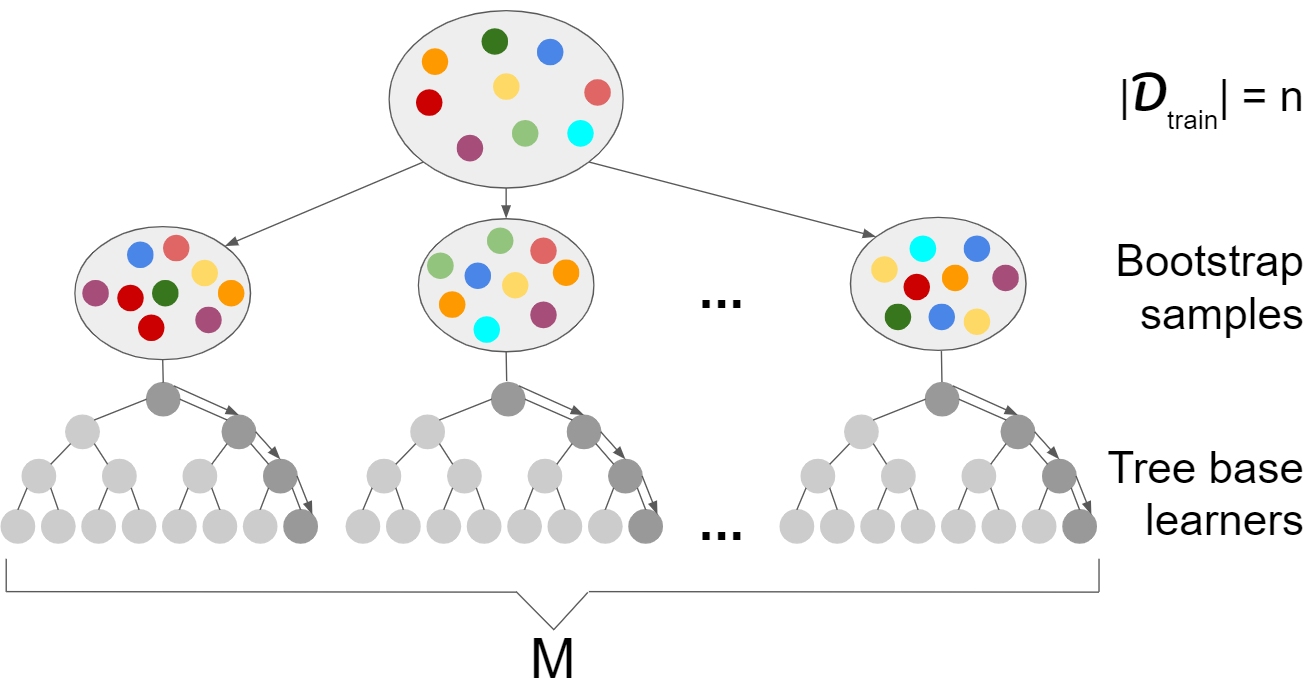
\includegraphics[width=0.6\textwidth]{figure/rf-bagging} \\
  \tiny Schematic depiction of bagging process
\end{minipage}%
\begin{minipage}[b]{0.35\textwidth}
\centering
  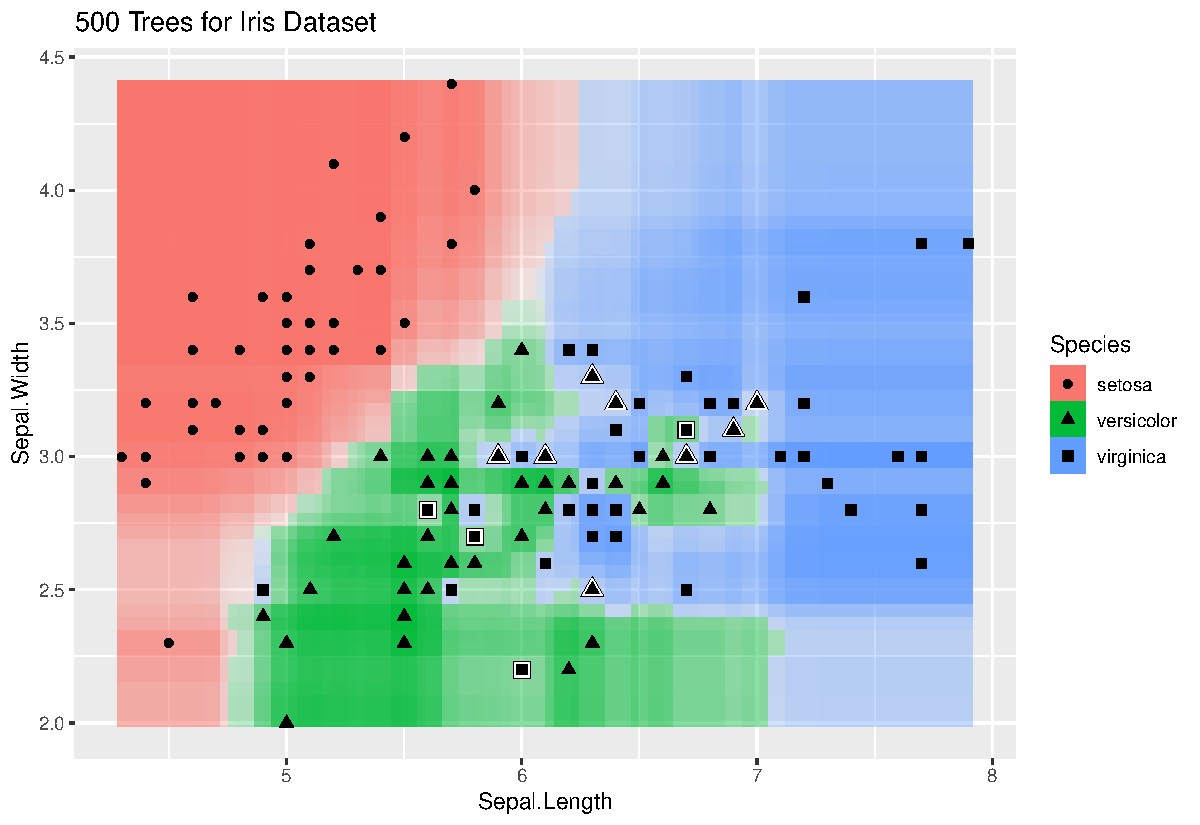
\includegraphics[width=0.9\textwidth]{
  ../slides/forests/figure/cart_forest_intro_3} \\
  \tiny Prediction surface for \texttt{iris} data with 500-tree ensemble
\end{minipage}

\end{frame}

% ------------------------------------------------------------------------------

\begin{frame}{Random Forests -- method summary}

\highlight{Empirical risk} (just like tree base learners)

\begin{itemize}
  \item In general, compatible with arbitrary losses
  \item Computation of empirical risk for all potential child nodes of all trees
\end{itemize}

\medskip

\highlight{Optimization} (just like tree base learners)

\begin{itemize}
    \item \textbf{Exhaustive} search over all split candidates choice of risk-minimal split (greedy optimization)
    \item Base learners can be fitted independently of each other (in parallel)
\end{itemize}

\medskip

\highlight{Hyperparameters}

\begin{itemize}
  \item \textbf{Ensemble size}, i.e., number of trees
  \item \textbf{Complexity} of base learners
  \item \textbf{Number of split candidates}, i.e., number of features to be
  considered at each split \\
  $\Rightarrow$ frequently used heuristics with total of $p$ features: 
  $\left \lfloor{\sqrt{p}}\right \rfloor$ for classification,
  $\left \lfloor{p/3}\right \rfloor$ for regression
\end{itemize}

\medskip

\highlight{Out-of-bag (OOB) error}
\begin{itemize}
  \item Ensemble prediction for obs. outside individual trees' bootstrap training sample $\Rightarrow$ unseen test sample
  \item Use resulting loss as unbiased estimate of \textbf{generalization error}
\end{itemize}

% \highlight{Runtime behavior} ~~
% $\mathcal{O}(M \cdot n^2 \cdot p)$ for $M$ trees, $n$ observations and $p$ 
% features
  
\end{frame}

% ------------------------------------------------------------------------------

\begin{frame}{Random Forests -- Pro's \& Con's}

\begin{columns}[onlytextwidth]
  \begin{column}{0.5\textwidth}
    \highlight{Advantages}
    \footnotesize
    \begin{itemize}
      \positem Retains most of \textbf{trees'} advantages (e.g., feature selection, feature interactions)
      \positem Fairly \textbf{good predictor}: mitigating base learners' weakness through bagging
      \positem Quite \textbf{robust} w.r.t. small changes in data
      \positem Good with \textbf{high-dimensional} data, even in presence of noisy features
      % \positem Applicable to \textbf{unbalanced} data
      \positem Easy to \textbf{parallelize}
      \positem Robust to its hyperparameter configuration
      \positem Intuitive measures of \textbf{feature importance}
    \end{itemize}
  \end{column}
  \begin{column}{0.5\textwidth}
    \highlight{Disadvantages}
    \footnotesize
    \begin{itemize}
      \negitem Loss of individual trees' \textbf{interpretability}
      \negitem Often suboptimal for \textbf{regression}
      \negitem \textbf{Bias} toward selecting features with many categories
      \negitem Rather large model size and slow inference time for large ensembles
      \negitem Typically inferior in \textbf{performance} to tuned gradient tree boosting.
    \end{itemize}
  \end{column}
\end{columns}

\vfill

\small

\conclbox{Fairly good and stable predictor with built-in feature selection, but 
black-box method}

\end{frame}

% ------------------------------------------------------------------------------

\begin{frame}{Random Forests -- Practical hints}

\highlight{Pre-processing} ~~ Inherent feature selection, but high 
\textbf{computational cost} for large number of features \\
$\Rightarrow$ upstream feature selection (e.g., via PCA) might be advisable

\medskip

\highlight{Feature importance}

\begin{itemize}
  \item Based on \textbf{improvement in split criterion:} aggregate improvements 
  by all splits using $j$-th feature
  \item Based on \textbf{permutation:} permute $j$-th feature in 
  OOB observations and compute impact on OOB error
\end{itemize}

\medskip

\highlight{Tuning} ~~ Number of split candidates often more impactful than 
number of trees

\medskip

\highlight{Implementation}

\begin{itemize}
  \item \textbf{R:} \texttt{mlr3} learners \texttt{LearnerClassifRanger} / 
    \texttt{LearnerRegrRanger}, calling \texttt{ranger::ranger()}
  \item \textbf{Python:} \texttt{RandomForestClassifier} / 
  \texttt{RandomForestRegressor} from package \texttt{scikit-learn}
\end{itemize}

\end{frame}

\section{Gradient Boosting}
\begin{frame}{Gradient Boosting -- method summary}

% \maketag{supervised} 
\maketag{regression} \maketag{classification}
\maketag[50]{(NON)PARAMETRIC}
\maketag{BLACK-BOX}
\maketag{FEATURE SELECTION}

\medskip

\highlight{General idea}

\begin{itemize}
  \item \textbf{Sequential ensemble} of $M$ \textbf{base learners} by greedy forward stagewise additive modeling
  \begin{itemize}
      \item In each iteration a base learner is fitted to current \textbf{pseudo residuals} $\Rightarrow$ one boosting iteration is one approximate \textbf{gradient step in function space}
      \item Base learners are either \textbf{trees} or \textbf{linear regressions}
  \end{itemize}
  \item \textbf{Predict} via (weighted) sum of base learners
  
\end{itemize}

\medskip

\highlight{Hypothesis space} ~~
$\Hspace = \left\{ \fx: \fx = \sum_{m = 1}^M \betam b(\xv, \thetam) \right\}$

\begin{minipage}{0.45\textwidth}
  \centering
  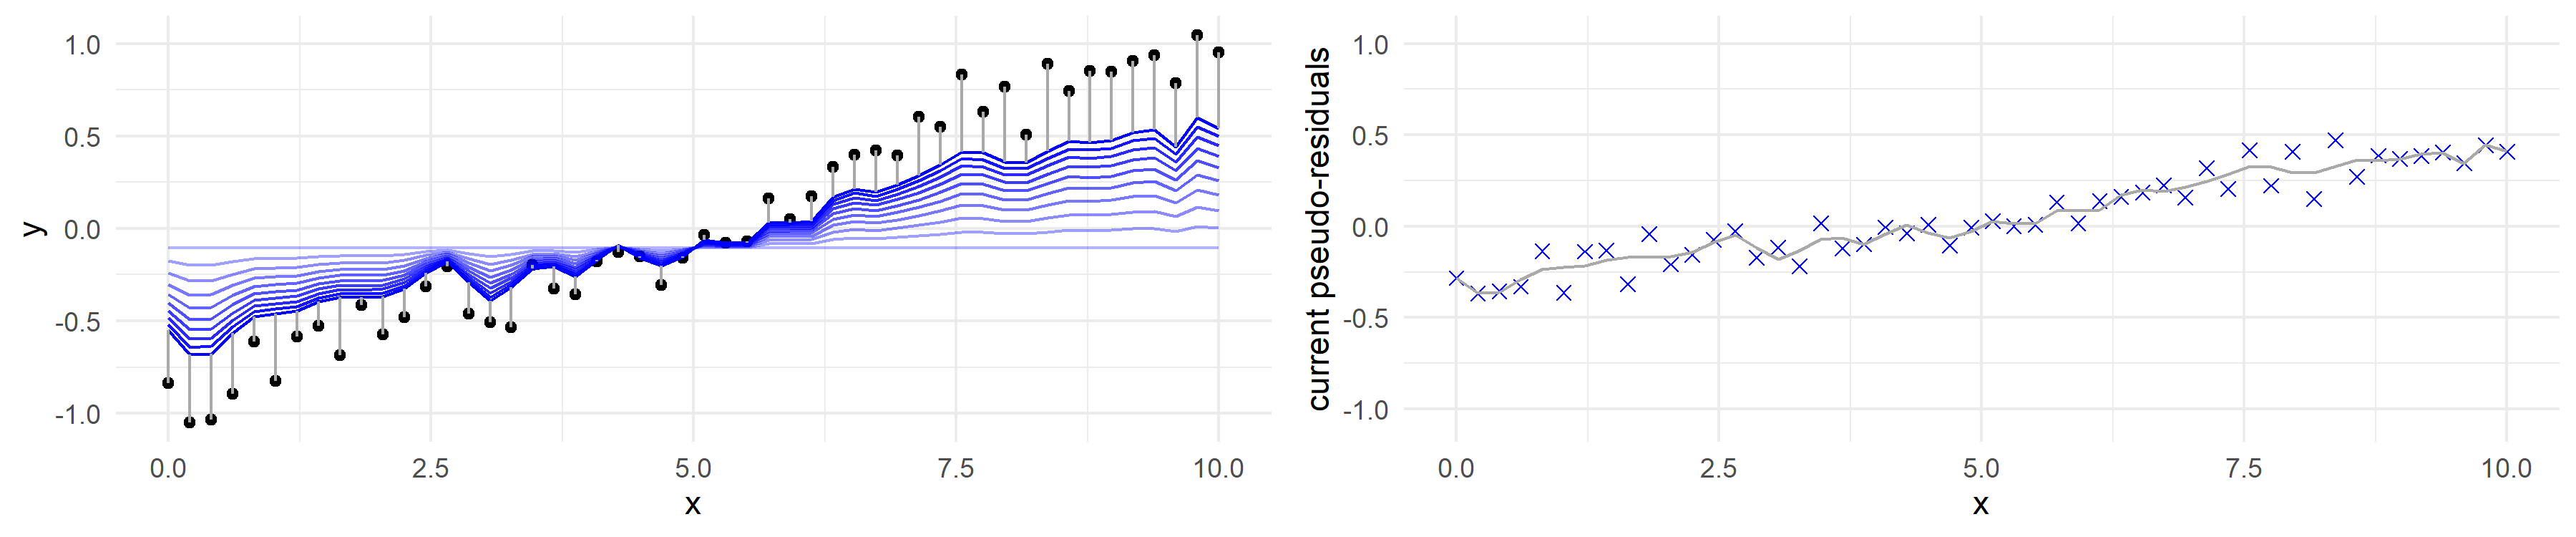
\includegraphics[width=\textwidth, trim=0 0 450 0, clip]{
  figure/illustration_gaussian_huber_2_10} \\
  \tiny{Boosting prediction function with GAM base learners for univariate 
  regression problem after 10 iterations}
\end{minipage}%
\hfill
\begin{minipage}{0.45\textwidth}
  % FIGURE SOURCE: http://arogozhnikov.github.io/2016/06/24/gradient_boosting_explained.html
  % 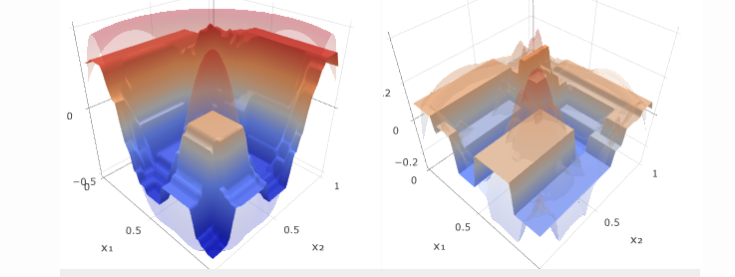
\includegraphics[width=\textwidth]{figure/gb-3d} \\
  \centering
  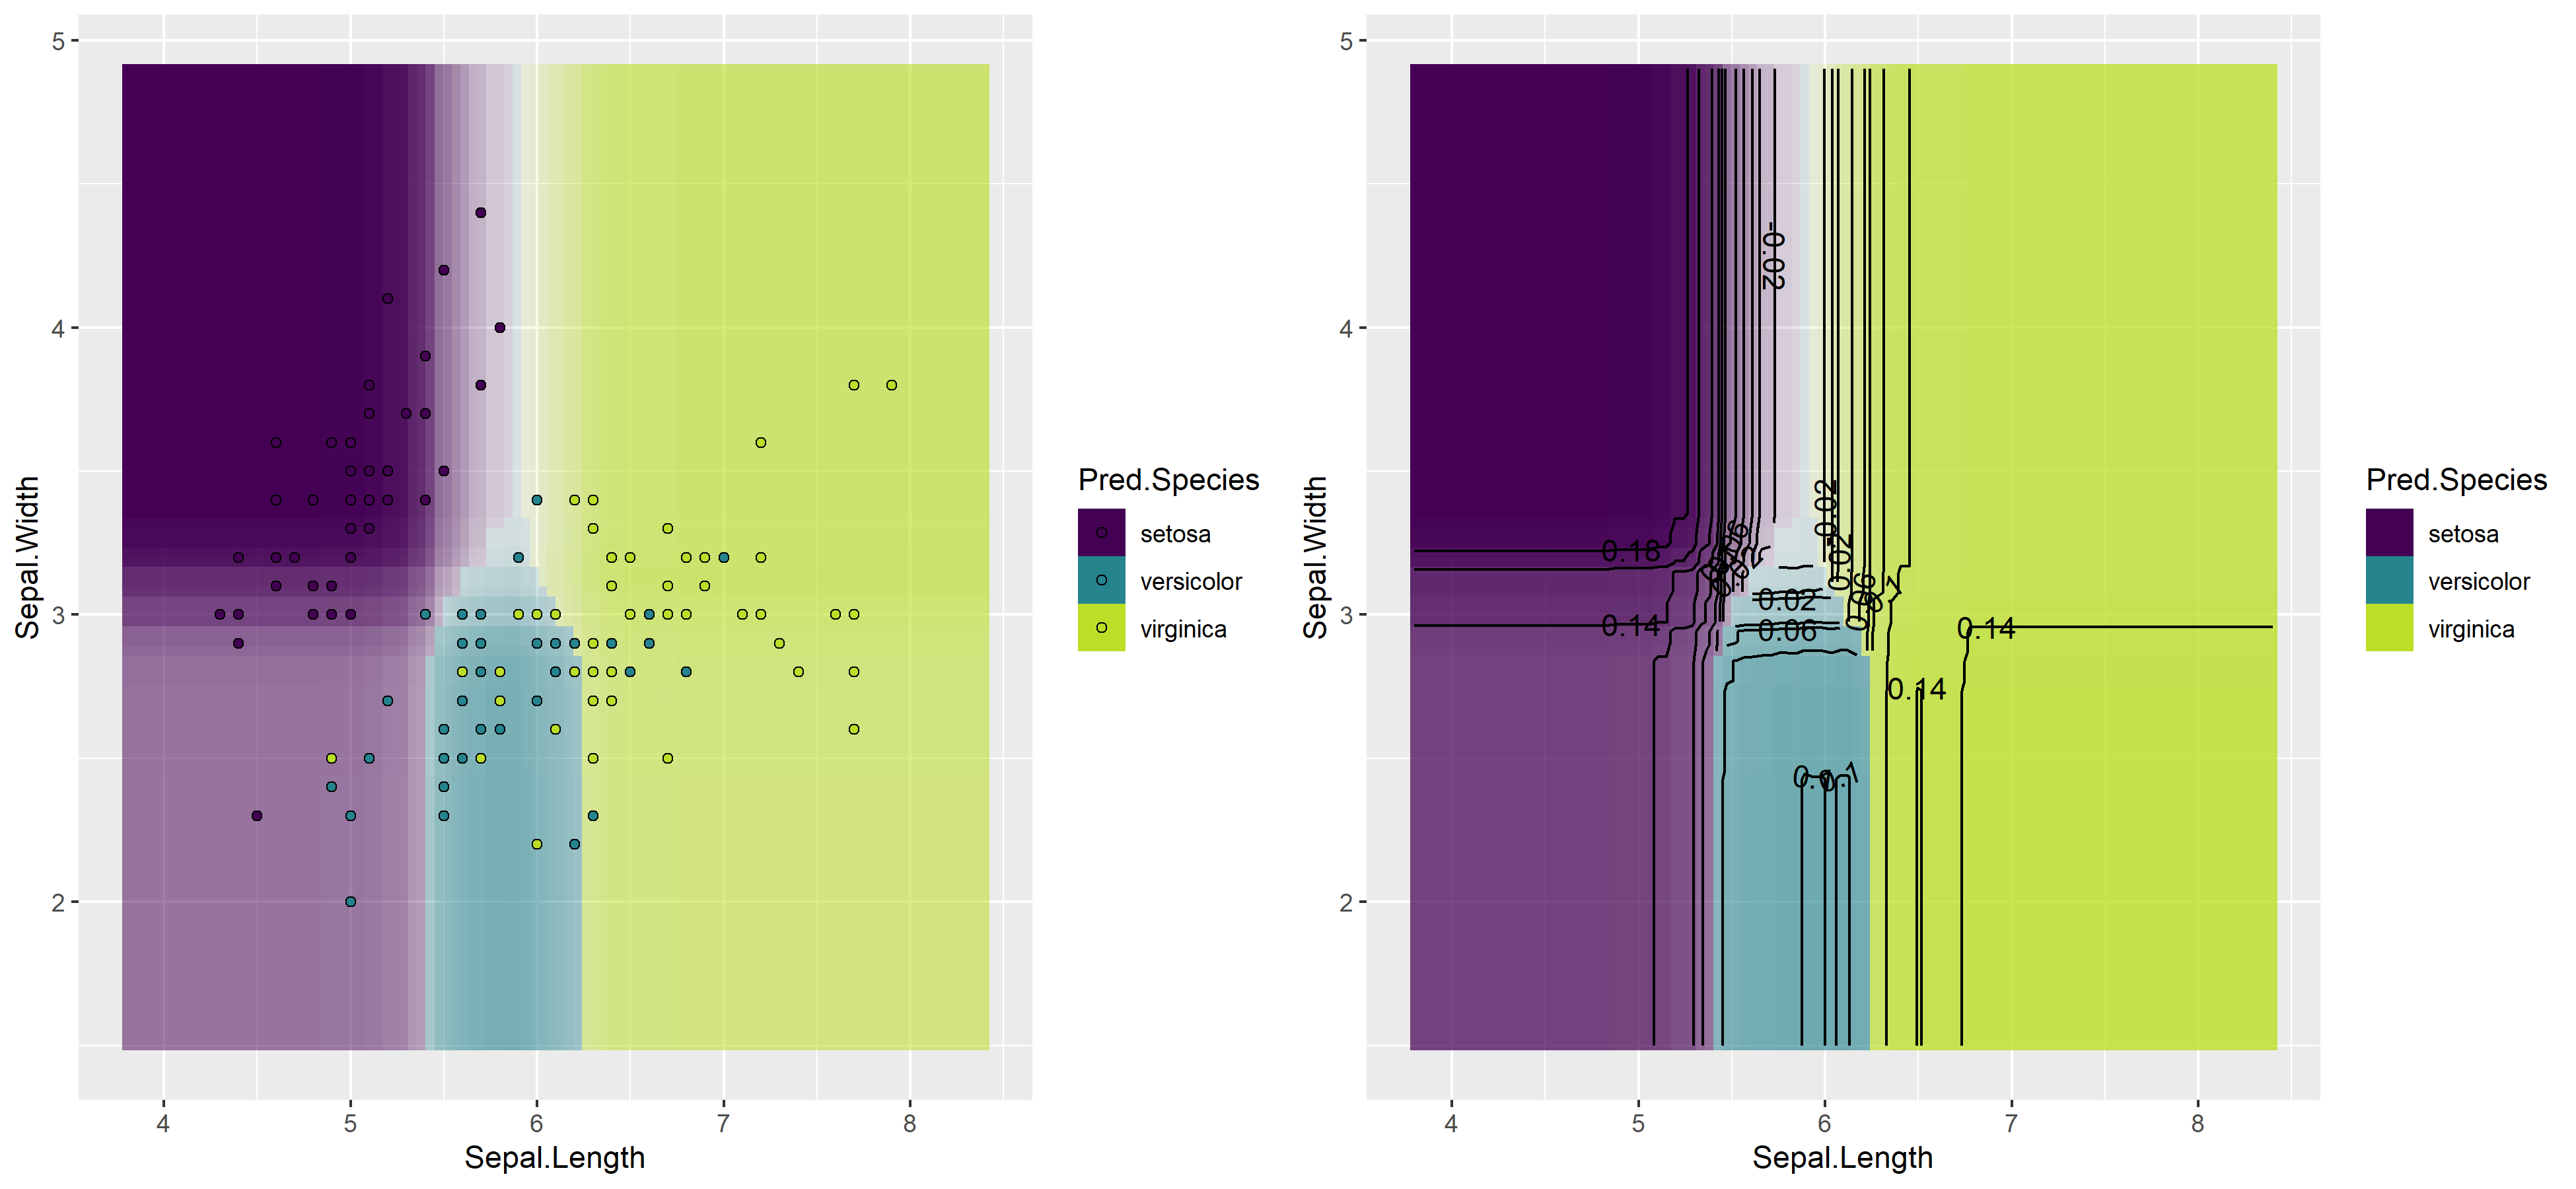
\includegraphics[width=\textwidth]{
  figure/boosting_multiclass_100} \\
  \tiny{Boosting prediction surface with tree base learners for \texttt{iris} 
  data after 100 iterations (\textit{right:} contour lines of discriminant 
  functions)}
\end{minipage}

\end{frame}

% ------------------------------------------------------------------------------

\begin{frame}{Gradient Boosting -- method summary}

\footnotesize

\highlight{Empirical risk}

\begin{itemize}
  \item In general, compatible with any \textbf{differentiable} loss
  \item Base learner in iteration $m$ is fitted on \textbf{Pseudo residuals}: $\tilde{r}^{(i)} = - \pd{\Lxyi}{\fxi}$ by minimizing the \textbf{L2-loss}: $\sumin (\rmi - b(\xi, \bm{\theta}))^2$
\end{itemize}

\medskip

\highlight{Optimization} ~~
\begin{itemize}
    \item Same optimization procedure as base learner, while keeping the current ensemble $\fmdh$ fixed
    \item $\betam$ is found via \textbf{line search} or fixed to a \textbf{small constant value} and combined with the leaf values $\ctm$ for tree base learners: $\ctmt = \betam \cdot \ctm$
\end{itemize}

\medskip

\highlight{Hyperparameters}

\begin{itemize}
  \item \textbf{Ensemble size}, i.e., number of base learners
  \item \textbf{Complexity} of base learners (depending on type used)
  \item \textbf{Learning rate}, i.e., impact of next base learner
\end{itemize}

\medskip

% \highlight{Runtime behavior} ~~ $\mathcal{O}(M \cdot n \cdot p)$ 
% for $M$ base learners, $n$ observations and $p$ features

\end{frame}


% ------------------------------------------------------------------------------

\begin{frame}{Gradient Boosting -- Practical hints}

\footnotesize

\highlight{Scalable Gradient Boosting} 

\begin{itemize}
  \item \textbf{Feature and data subsampling} for each base learner fit
  \item \textbf{Parallelization} and \textbf{approximate split finding} for tree base learners
  \item GPU accelaration
\end{itemize}

\medskip

\highlight{Explainable / Componentwise Gradient Boosting}
\begin{itemize}
    \item Base learners of \textbf{simple linear regression} models or \textbf{splines}, selecting a single feature in each iteration
    \item Allows \textbf{feature selection} and creates an \textbf{interpretable} model
    \item Feature interactions can be learned via ranking techniques (e.g., GA$^2$M FAST)
\end{itemize}

\medskip

\highlight{Tuning}
\begin{itemize}
    \item Use \textbf{early-stopping} to determine ensemble size
    \item Tune learning rate and base learner complexity hyperparameters on \textbf{log-scale}
\end{itemize}

\medskip

\highlight{Implementation}

\begin{itemize}
  \item \textbf{R:} \texttt{mlr3} learners \texttt{LearnerClassifXgboost} / 
  \texttt{LearnerRegrXgboost}, calling \texttt{xgboost::xgb.train()}
  \item \textbf{Python:} \texttt{GradientBoostingClassifier} / 
  \texttt{GradientBoostingRegressor} from package \texttt{scikit-learn}, 
  \texttt{XGBClassifier} / \texttt{XGBRegressor} from package \texttt{xgboost}
\end{itemize}

\end{frame}


% ------------------------------------------------------------------------------

\begin{frame}{Gradient Boosting -- Pro's \& Con's}

\footnotesize

\begin{columns}[onlytextwidth]
  \begin{column}{0.5\textwidth}
    \highlight{Advantages}
    \footnotesize
    \begin{itemize}
      \positem Retains of most of \textbf{base learners'} advantages 
      \positem Very \textbf{good predctor}: mitigating base learners' weakness through ensembling
      \positem Often state-of-the-art results, only outperformed by heterogenous \textbf{stacking ensembles}
      \positem High \textbf{flexibility} via custom loss functions and choice of base learner
      % \positem Applicable to \textbf{unbalanced} data
    \end{itemize}
  \end{column}
  \begin{column}{0.5\textwidth}
    \highlight{Disadvantages}
    \footnotesize
    \begin{itemize}
      \negitem Loss of base learners' potential \textbf{interpretability}
      \negitem \textbf{Many hyperparameters} that need to be tuned carefully
      \negitem Hard to \textbf{parallelize}
    \end{itemize}
  \end{column}
\end{columns}

\vfill

\small

\conclbox{High-performing and flexible predictor, but rather delicate to handle}

\end{frame}

\section{Linear Support Vector Machines (SVM)}
\begin{vbframe}{Linear SVM -- Functionality}

% \maketag{SUPERVISED} 
\maketag{CLASSIFICATION} \maketag{PARAMETRIC} 
\maketag{BLACK-BOX} 
\medskip

\highlight{General idea}

\begin{itemize}
  \item Find linear decision boundary (\textbf{separating hyperplane}) that 
  best separates classes
  \begin{itemize}
    \item \textbf{Hard-margin} SVM: maximize distance (\textbf{margin} 
    $\gamma$ > 0) to closest members (\textbf{support vectors, SV}) on each 
    side of decision boundary
    \item \textbf{Soft-margin} SVM: relax separation to allowing margin 
    violations $\rightarrow$ maximize margin while minimizing violations
  \end{itemize}
  \item 3 types of training points
  \begin{itemize}
    \item \textbf{non-SVs} with no impact on decision boundary
    \item \textbf{SVs} located exactly on decision boundary
    \item \textbf{margin violators}
  \end{itemize}
\end{itemize}

\medskip

\highlight{Hypothesis space} ~~
$\Hspace = \left\{f: \Xspace \to \R ~|~\fx = \thetab^\top \xv + \theta_0
\right\}$
 ~~ \textcolor{blue}{separater intercept notwendig?}

\framebreak

\medskip
\footnotesize
\begin{minipage}{0.6\textwidth}
  \centering
  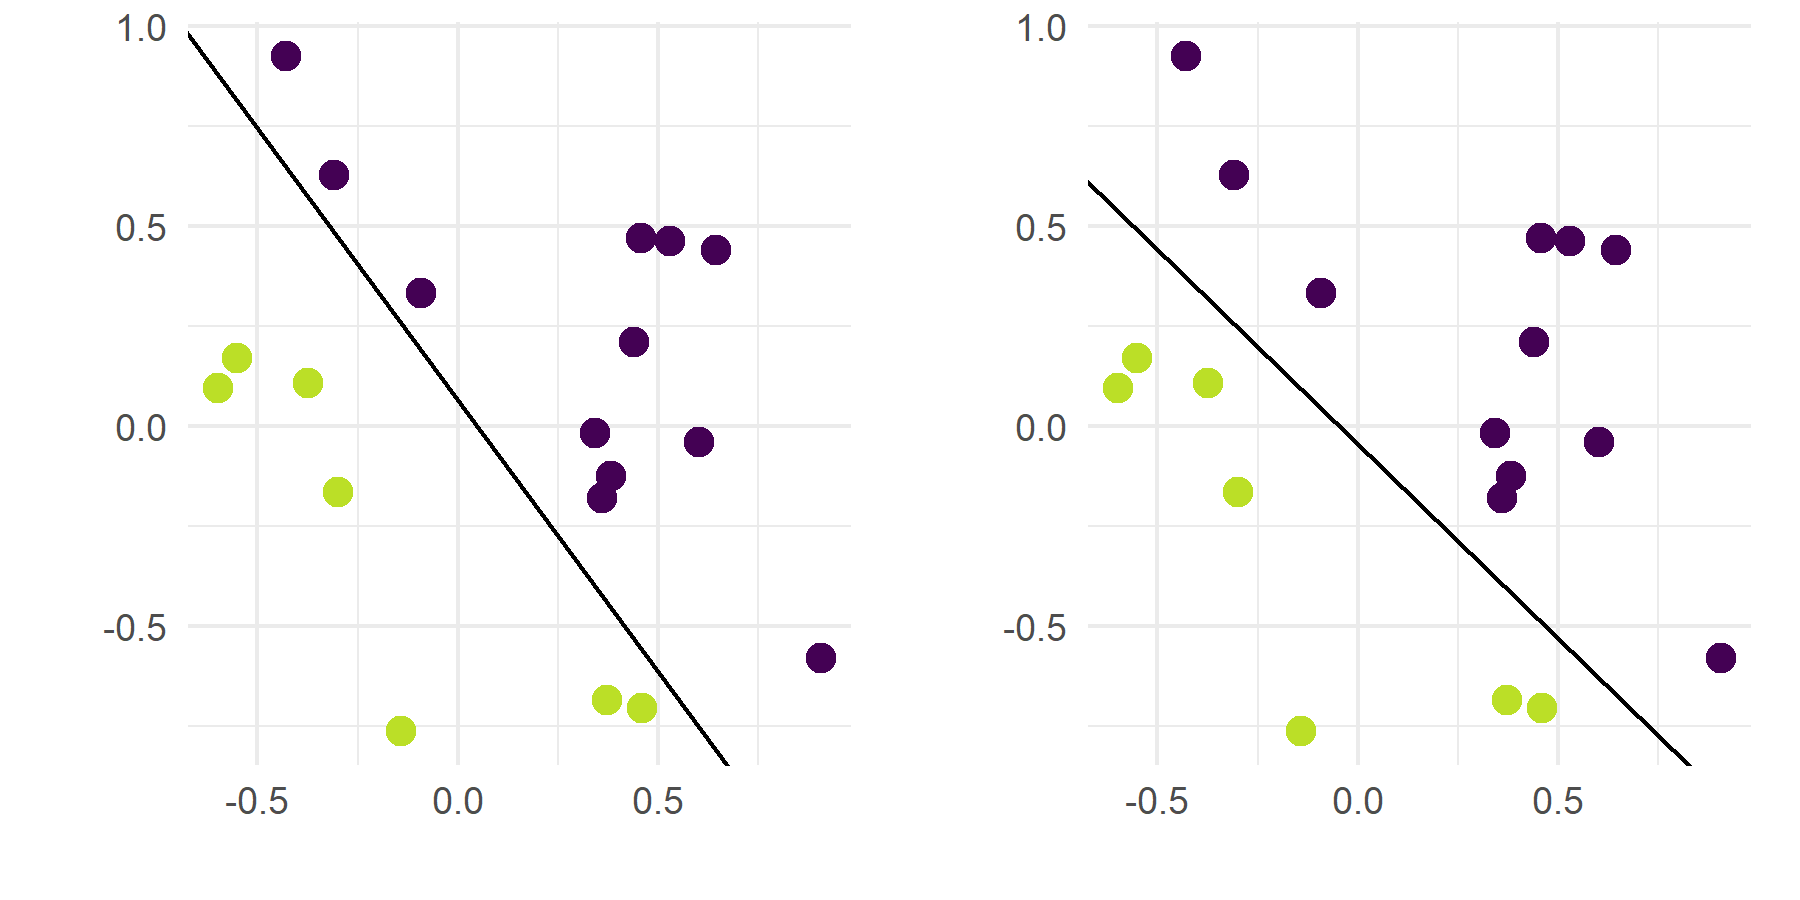
\includegraphics[width=0.9\textwidth]{
  ../slides/linear-svm/figure/linear_classif_1.png}  \\
  \tiny{Hard-margin SVM: margin is maximized by boundary on the right}
\end{minipage}
\hfill
\begin{minipage}{0.3\textwidth}
  \centering
    %https://docs.google.com/presentation/d/1g7q1hbTNmQeuRWQIM8SF9l6iKWmJyuhyhm3s9QjA0jM/edit?usp=sharing
  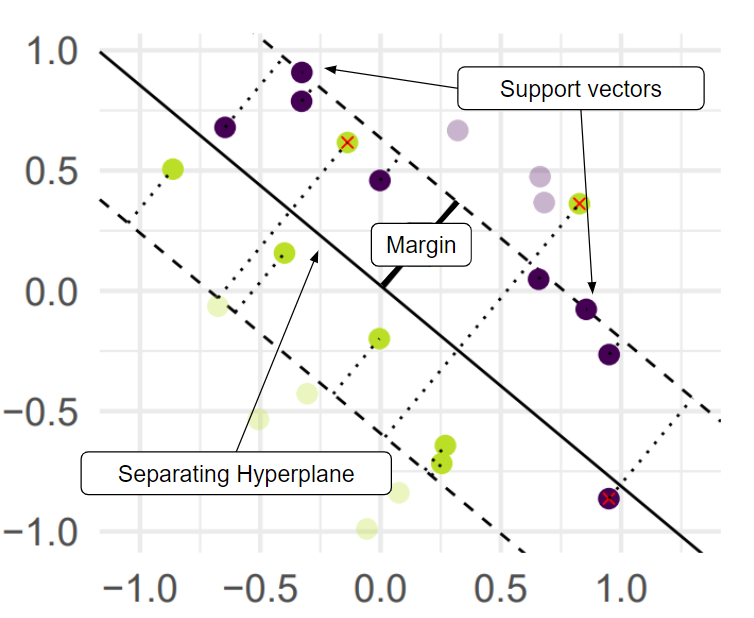
\includegraphics[width=1.1\textwidth]{figure/svm_wording.png} \\
  \tiny{Soft-margin SVM with margin violations}
\end{minipage}

\medskip

\highlight{Dual problem} ~~ %lecture_cim2\2020\08-linear-svm\slides-3-soft-margin-svm.Rnw
\begin{eqnarray*}
    & \max\limits_{\alphav \in \R^n} & \dualobj \\
    & \text{s.t. } & 0 \le \alpha_i \le C ~~ \forall i \in \nset ~~ (C = \infty
    \text{ for hard-margin SVM)}, \\
    & \quad & \sum_{i=1}^n \alpha_i \yi = 0
\end{eqnarray*}

\framebreak

\highlight{Empirical risk}

Soft-margin SVM also interpretable as \textbf{L2-regularized ERM}: 

\begin{minipage}[b]{0.58\textwidth}
  $$ \frac{1}{2} \|\thetab\|^2 + C \sumin \Lxyi$$ 
  with  
  \begin{itemize}
    \item $\|\thetab\| = 1 / \gamma$,\\
    \item $C > 0$: penalization for missclassified data points
    \item $\Lyf = \max(1-yf, 0)$: \textbf{hinge} loss \\
    $\rightarrow$ other loss functions applicable (e.g., \textbf{Huber} loss)
  \end{itemize}
\end{minipage}
\begin{minipage}[b]{0.4\textwidth}
  \centering
  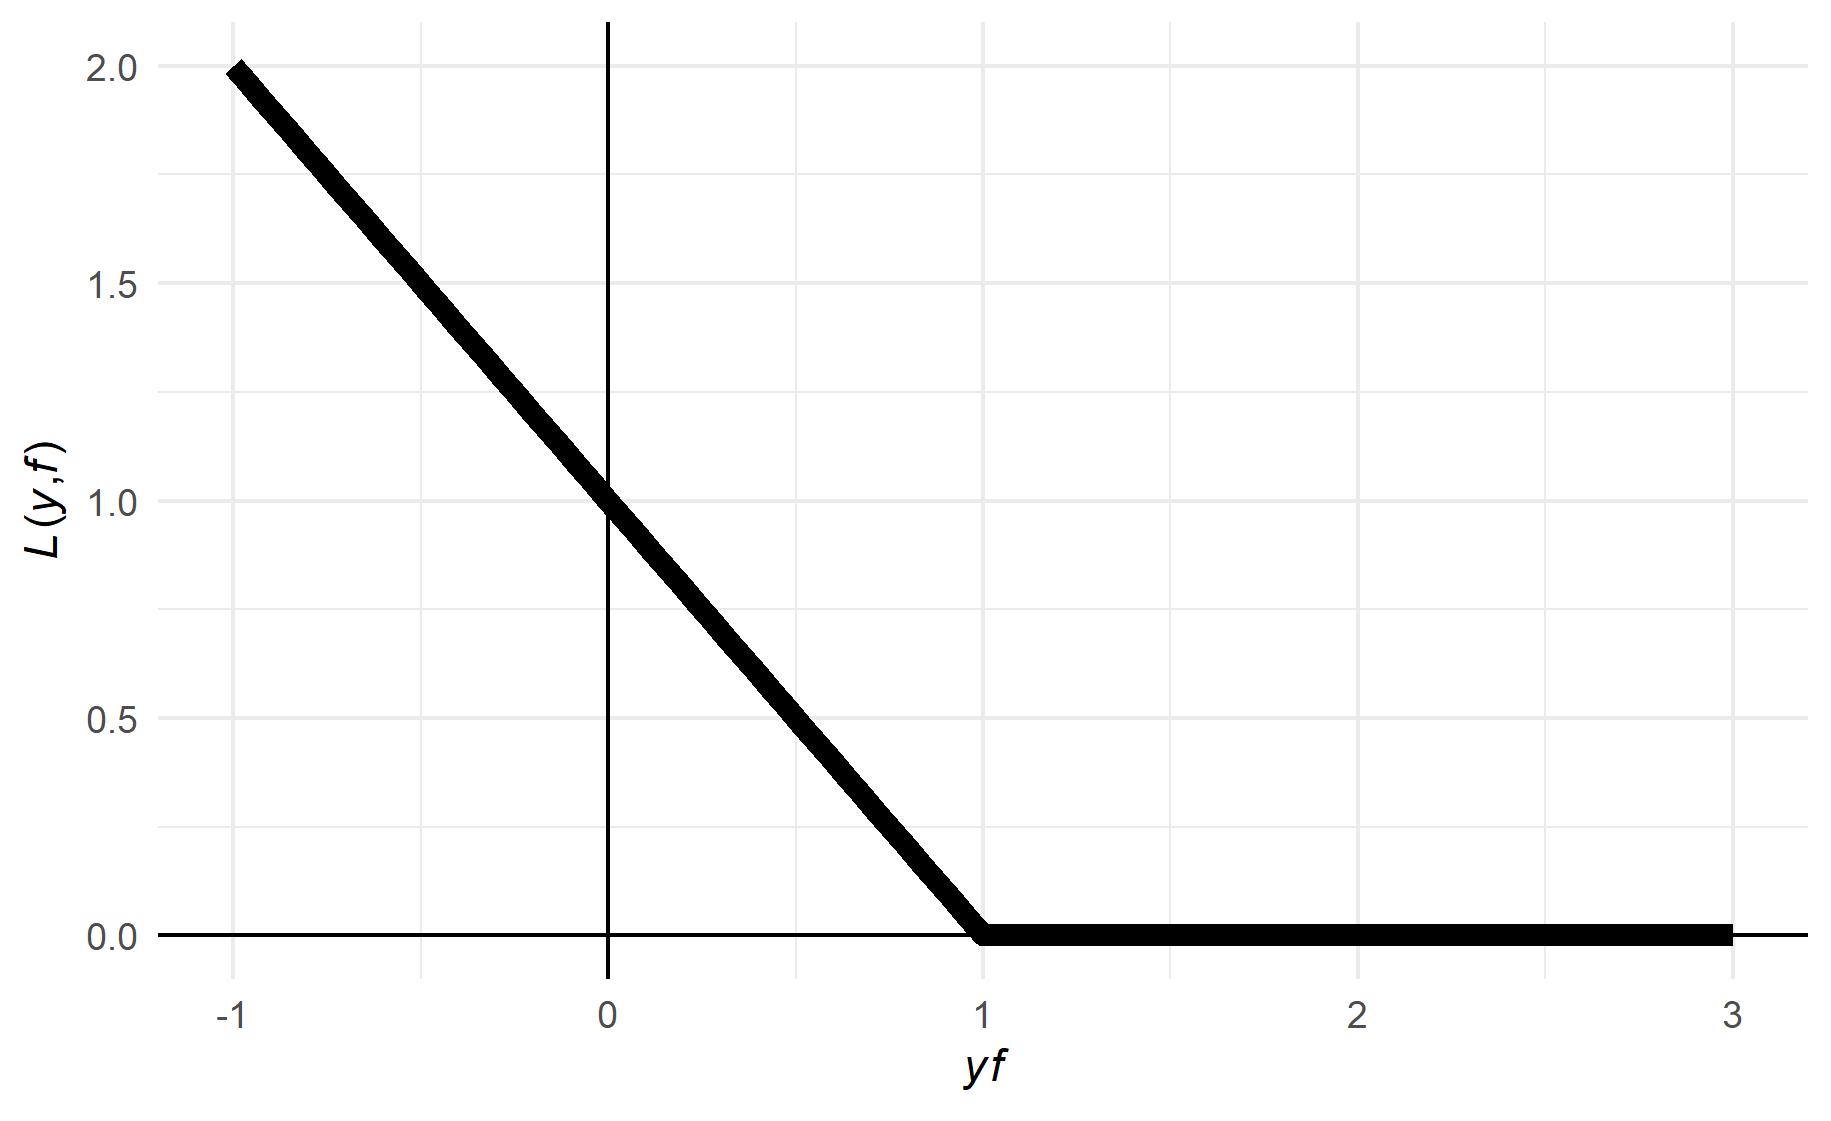
\includegraphics[height=0.4\textwidth, keepaspectratio=true]{
  figure/plot-hinge-loss.png}
\end{minipage}

\medskip

\highlight{Optimization}

\begin{itemize}
  \item Typically, tackling \textbf{dual} problem (though feasible 
  in corresponding primal) via \textbf{quadratic programming}
  \item Popular: \textbf{sequential minimal optimization} $\rightarrow$ 
  iterative algorithm based on breaking down objective into bivariate quadratic 
  problems with analytical solutions
\end{itemize}
\medskip

\highlight{Hyperparameters} ~~ Cost parameter \textbf{$C$}

\end{vbframe}

% ------------------------------------------------------------------------------

\setdraft

\begin{frame}{Linear SVM -- Pro's \& Con's}

\begin{columns}[onlytextwidth]
  \begin{column}{0.5\textwidth}
    \highlight{Advantages}
    \footnotesize
    \begin{itemize}
      % \positem High \textbf{accuracy}
      \positem Often \textbf{sparse} solution
      \positem Robust against overfitting (\textbf{regularized}); especially in 
      high-dimensional space
      \positem \textbf{Stable} solutions, as non-SV do not influence decision 
      boundary
      %\positem \textbf{memory efficient} (only use non-SVs)
    \end{itemize}
  \end{column}

  \begin{column}{0.5\textwidth}
    \highlight{Disadvantages}
    \footnotesize
    \begin{itemize}
      \negitem \textbf{Costly} implementation; long training times
      \negitem \textbf{Limited scalability} to larger data sets 
      \textcolor{blue}{\textbf{??}}
      \negitem Confined to \textbf{linear separation}
      \negitem Poor \textbf{interpretability}
      \negitem No handling of \textbf{missing} data
    \end{itemize}
  \end{column}
\end{columns}

\vfill

\small

\conclbox{Very accurate solution for high-dimensional data that is linearly separable}

\end{frame}

\undraft

% ------------------------------------------------------------------------------

\begin{frame}{Linear SVM -- Practical hints}

\footnotesize

  \highlight{Preprocessing} \\
  Features must be rescaled before applying SVMs.
  
  \medskip
  
  \highlight{Tuning} \\
  Cost parameter $C$ must be tuned and has strong influence on resulting 
  separating hyperplane. 

  \medskip

  \highlight{Implementation} 
  \begin{itemize}
    \item \textbf{R:} \texttt{mlr3} learners \texttt{LearnerClassifSVM} / 
    \texttt{LearnerRegrSVM}, calling \texttt{svm()} from \texttt{libsvm}
    \item \textbf{Python:} \texttt{sklearn.svm.SVC} from package 
    \texttt{scikit-learn} / package \texttt{libSVM}
  \end{itemize}

\end{frame}


\section{Nonlinear Support Vector Machines}
\begin{frame}{nonlinear SVM -- method summary}

\footnotesize

% \maketag{SUPERVISED} 
\maketag{CLASSIFICATION} \maketag[50]{REGRESSION} \maketag{NONPARAMETRIC} 
\maketag{BLACK-BOX}

\medskip

\highlight{General idea}
\begin{itemize}
  \item Move \textbf{beyond linearity} by mapping data to 
  transformed space where they are linearly separable
  \item \textbf{Kernel trick} %\textcolor{blue}{(based on Mercer's theorem,  existence of reproducing kernel Hilbert space)}: 
  \begin{itemize}
    % \item Replace two-step operation feature map $\phi$ $\leadsto$ inner product 
    % by \textbf{kernel} $k: \Xspace \times \Xspace \rightarrow \R$, s.t.
    % $\scp{\phix}{\phixt} = \kxxt$
    \item No need for explicit construction of feature maps
    \item Replace inner product of feature map $\phi$ by \textbf{kernel}: $\scp{\phix}{\phixt} = \kxxt$
  \end{itemize}
  %\item Loss of interpretability through nonlinear feature map
\end{itemize}


\medskip

% \operatorname{sign}(\mathbf{w} \cdot \Phi(\mathbf{x})+b)

\highlight{Hypothesis space} ~~
% $\Hspace = \left \{ \fx = \sumin \alpha_i \yi k(\xi, \xv)  + \theta_0 ~|~
% \theta_0, \alpha_i \in \R ~ \forall i \right \} $
%\textcolor{blue}{$\Hspace = \{ \operatorname{sign}(\sumin \alpha_i \yi k(\xi, \xv)  + \theta_0) |\ (\theta_0, \thetab) \in \R^{p+1} \} $}
%$\left \{ \fx = \sumin \alpha_i \yi  k(\xi, \xv)   +     \theta_0 ~|~ \alpha_i \geq 0 ~ \forall i \right \}$

$\Hspace  = \left \{\fx ~:~ \fx = \sign \left( \sumin \alpha_i \yi k(\xi, \xv) + \theta_0 \right) ~|~ \alpha_i \geq 0,  \sumin \alpha_i \yi = 0 \right \}$\\
$\Rightarrow$ \textbf{Note:} Non-SVs have $\alpha_i = 0$ as they do not affect the hyperplane

% \langle \phi \left( \xi \right), \phi(\xv) \rangle
\begin{columns}[c, totalwidth=\textwidth]
    \begin{column}{0.24\textwidth}
          \centering
  \includegraphics[width=0.8\textwidth]{
  figure/circles_ds.png} \\
  \tiny{Nonlinear problem in original space} 
    \end{column}
    \begin{column}{0.75\textwidth}
          \centering
  \includegraphics[width=0.9\textwidth, trim=0 30 0 50, clip]{
  figure/circles_feature_map.png} \\
  \tiny{Mapping to 3D space and subsequent linear separation -- implicitly handled by kernel in nonlinear SVM}
    \end{column}
\end{columns}

% \begin{minipage}[t]{0.33\textwidth}
%   \centering
%   \includegraphics[width=0.5\textwidth]{
%   figure/circles_ds.png} \\
%   \tiny{Nonlinear problem in original space} 
% \end{minipage}
% \begin{minipage}[t]{0.66\textwidth}
%   \centering
%   \includegraphics[width=0.9\textwidth, trim=0 30 0 0, clip]{
%   figure/circles_feature_map.png} \\
%   \tiny{Mapping to 3D space and subsequent linear separation -- implicitly 
%   handled by kernel in nonlinear SVM}
% \end{minipage}

\end{frame}

% ------------------------------------------------------------------------------

\begin{frame}{nonlinear SVM -- method summary}

\footnotesize

\highlight{Dual problem} ~~ \textbf{Kernelize} dual (soft-margin) SVM problem, 
replacing all inner products by kernels:
$$\max_{\alphav} \sumin \alpha_i - \frac{1}{2}\sumin \sumjn
\alpha_i\alpha_j\yi y^{(j)} \textcolor{blue}{k(\xi, \xi[j])}, ~~ \text{s.t. } ~~ 
0 \le \alpha_i \le C, ~~ \sumin \alpha_i \yi = 0.
$$

\medskip

\highlight{Hyperparameters} ~~ Cost $C$ of margin violations, kernel 
hyperparameters (e.g., width of RBF kernel)

\medskip

\begin{columns}[T, totalwidth=\textwidth]
    \begin{column}{0.59\textwidth}
        
\highlight{Interpretation as basis function approach}
  \begin{itemize}
    \item \textbf{Representer theorem:} solution of dual soft-margin SVM problem is
    $\thetab = \sum_{j=1}^n \beta_j \phi (\xi[j] )$ \\
    \item Sparse, weighted sum of \textbf{basis functions}\\
    $\rightarrow \beta_j = 0$ 
    for non-SVs
    \item Result: \textbf{local} model with smoothness depending on kernel
  \end{itemize}
    \end{column}
        \begin{column}{0.4\textwidth}
        \centering
  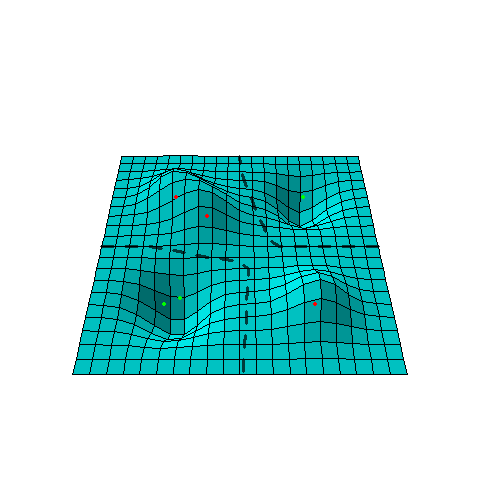
\includegraphics[width=\textwidth, trim=50 100 50 150, clip]{
  figure/svm_rbf_as_basis.png} \\
  \tiny{RBF kernel as mixture of Gaussian basis functions, forming
  bumpy, nonlinear decision surface to discern red and green points}
    \end{column}
\end{columns}

\end{frame}

% ------------------------------------------------------------------------------

\begin{frame}{nonlinear SVM -- Practical hints}

\footnotesize

\highlight{Common kernels}

\begin{itemize}
  \item \textbf{Linear} kernel: dot product of given observations ~~ 
  $\Rightarrow \kxxt = \xv^\top \xtil$ ~~ $\Rightarrow$ linear SVM
  \item \textbf{Polynomial} kernel of degree $d \in \N$: monomials (i.e., 
  feature interactions) up to $d$-th 
  order ~~$\Rightarrow 
  \kxxt = \left(\xv^\top \xtil + b \right)^d, ~ b \geq 0$
  \item \textbf{Radial basis function (RBF)} kernel: infinite-dimensional 
  feature space, allowing for perfect separation of all finite 
  datasets ~~ $\Rightarrow \kxxt = \exp \left( -\gamma \| \xv - \xtil \|_2^2 
  \right )$ with 
  bandwidth parameter $\gamma > 0$
\end{itemize}
 
\medskip

 \highlight{Tuning}
 
 \begin{itemize}
  \item High sensitivity w.r.t. hyperparameters, especially those of kernel
  ~~ $\Rightarrow$ \textbf{tuning} very important
  \item For RBF kernels, use \textbf{RBF sigma heuristic} to determine 
  bandwidth
\end{itemize}

  \medskip

\highlight{Implementation} 
\begin{itemize}
  \item \textbf{R:} \texttt{mlr3} learners \texttt{LearnerClassifSVM} /
  \texttt{LearnerRegrSVM}, calling \texttt{e1071::svm()} with nonlinear kernel (\texttt{libSVM} interface),
  \texttt{kernlab::ksvm()} allowing custom kernels
  \item \textbf{Python:} \texttt{sklearn.svm.SVC} from package 
  \texttt{scikit-learn} / package \texttt{libSVM}
\end{itemize}

\end{frame}
% ------------------------------------------------------------------------------


% ------------------------------------------------------------------------------

\begin{frame}{SVM -- Pro's \& Con's}

\begin{columns}[T, totalwidth=\textwidth]
  \begin{column}{0.5\textwidth}
    \highlight{Advantages}
    \footnotesize
    \begin{itemize}
      % \positem High \textbf{accuracy}
      \positem Often \textbf{sparse} solution (w.r.t. observations)
      \positem Robust against overfitting (\textbf{regularized}); especially in 
      high-dimensional space
      \positem \textbf{Stable} solutions (w.r.t. changes in train data)\\
      $\rightarrow$ Non-SV do not affect decision boundary
      \positem Convex optimization problem \\
      $\rightarrow$ local minimum $\hat{=}$ global minimum
      %\positem \textbf{memory efficient} (only use non-SVs)
    \end{itemize}
    
    % \highlight{Advantages (nonlinear SVM)}
    % \begin{itemize}
    %    \positem Can learn \textbf{nonlinear decision boundaries}
    %    \positem \textbf{Very flexible} due to custom kernels \\
    %    $\rightarrow$ RBF kernel yields local model \\
    %    $\rightarrow$ kernel for time series, strings etc.
    % \end{itemize}
  \end{column}

  \begin{column}{0.5\textwidth}
    \highlight{Disadvantages}
    \footnotesize
    \begin{itemize}
      \negitem \textbf{Long} training times $\rightarrow O(n^2 p + n^3)$
      %\negitem \textbf{Limited scalability} to larger data sets 
      %\textcolor{blue}{\textbf{??}}
      \negitem Confined to \textbf{linear model}
      \negitem Restricted to \textbf{continuous features}
      \negitem Optimization can also fail or get stuck
      % \negitem Poor \textbf{interpretability}
      %\negitem No handling of \textbf{missing} data
    \end{itemize}

    %     \highlight{Disadvantages (nonlinear SVM)}
    % \begin{itemize}
    %    \negitem Poor \textbf{interpretability} due to complex kernel
    %    \negitem \textbf{Not easy tunable} as it is highly important to choose the right kernel (which also introduces further hyperparameters)
    % \end{itemize}
  \end{column}
\end{columns}



\begin{columns}[b, totalwidth=\textwidth]
  \begin{column}{0.5\textwidth}    
    \highlight{Advantages (nonlinear SVM)}
    \begin{itemize}
       \positem Can learn \textbf{nonlinear decision boundaries}
       \positem \textbf{Very flexible} due to custom kernels \\
       $\rightarrow$ RBF kernel yields local model \\
       $\rightarrow$ kernel for time series, strings etc.
    \end{itemize}
  \end{column}

  \begin{column}{0.5\textwidth}

        \highlight{Disadvantages (nonlinear SVM)}
    \begin{itemize}
       \negitem Poor \textbf{interpretability} due to complex kernel
       \negitem \textbf{Not easy tunable} as it is highly important to choose the right kernel (which also introduces further hyperparameters)
    \end{itemize}
  \end{column}
\end{columns}
\vfill

\small

\conclbox{nonlinear SVMs perform very well for nonlinear separable data, but are  hard to interpret and need a lot of tuning.}

% \conclbox{Very accurate solution for high-dimensional data that is linearly 
% separable}

\end{frame}

% \begin{frame}{nonlinear SVM -- Pro's \& Con's}

% \footnotesize

% \begin{columns}[onlytextwidth]
%   \begin{column}{0.5\textwidth}
%     \highlight{Advantages}
%     \footnotesize
%     \begin{itemize}
%       %\positem high \textbf{accuaracy}
%       \positem Can learn \textbf{nonlinear decision boundaries}
%       \positem Often \textbf{sparse} solution (w.r.t. observations)
%       \positem Robust against overfitting (\textbf{regularized}); especially in 
%       high-dimensional space 
%       \item \textbf{Stable} solutions (w.r.t. changes in train data)\\
%       $\rightarrow$ Non-SV do not affect decision boundary
%       \positem \textbf{Very flexible} due to custom kernels \\
%       $\rightarrow$ kernel for time series, strings etc.
%     \end{itemize}
%   \end{column}

%   \begin{column}{0.5\textwidth}
%     \highlight{Disadvantages}
%     \footnotesize
%     \begin{itemize}
%       \negitem \textbf{Costly} implementation; long training times
%       %\negitem does not scale well to \textbf{larger data sets} 
%       %\textcolor{blue}{\textbf{??}}
%       \negitem Poor \textbf{interpretability} due to complex kernel
%       %\item[$\textbf{\textcolor{gray!80}{-}}$] very memory-intensive
%       \negitem \textbf{Not easy tunable} as it is highly important to choose the 
%       right kernel
%       %\negitem No handling of \textbf{missing} data
%     \end{itemize}
%   \end{column}
% \end{columns}

% \vfill

% \small

% \conclbox{nonlinear SVMs perform very well for nonlinear separable data, but are 
% hard to interpret and need a lot of tuning.}

% \end{frame}


% \section{Gaussian Processes (GP)}
% %! Author = Son Trinh
%! Date = 10/13/2022

\begin{frame}{Gaussian Processes (GP) -- method summary}

\maketag{regression} \maketag{classification} \maketag{nonparametric} \maketag{probabilistic}

\medskip

\highlight{General idea}
\begin{itemize}
  \item GPs model a distribution over potential functions $\bm{f}$ that fit the observed data
  \item \textbf{Assumptions}:
  \begin{itemize}
     \item $n$-observations follow a $n$-dimensional Normal distribution
     \item The closer observations are, the higher they are correlated
  \end{itemize}
  \item A \textbf{kernel} function $k(\xi, \xv^{(j)})$ quantifies the similarity between two observations and induced the coviariance matrix of the distribution. 
  \item \textbf{Predict} via the maximum a-posteriori (MAP) estimate.
\end{itemize}

\medskip

\highlight{Hypothesis space} ~~
$\Hspace = \left\{ \bm{f} = \left[f\left(\xi[1]\right), \dots, f\left(\xi[n]\right)\right] \sim \mathcal{N}\left(\bm{m}, \bm{K}\right) ~|~ \bm{m} \in \R^n, \bm{K} \in \R^{n\times n} \right\}$

\medskip

\begin{minipage}[b]{0.5\textwidth}
  % FIGURE SOURCE: https://docs.google.com/presentation/d/1xodP6ayu1Gay6mMKgzVWYEFmSoeG5kNuqsaTkFFmd78  /edit
  \centering
  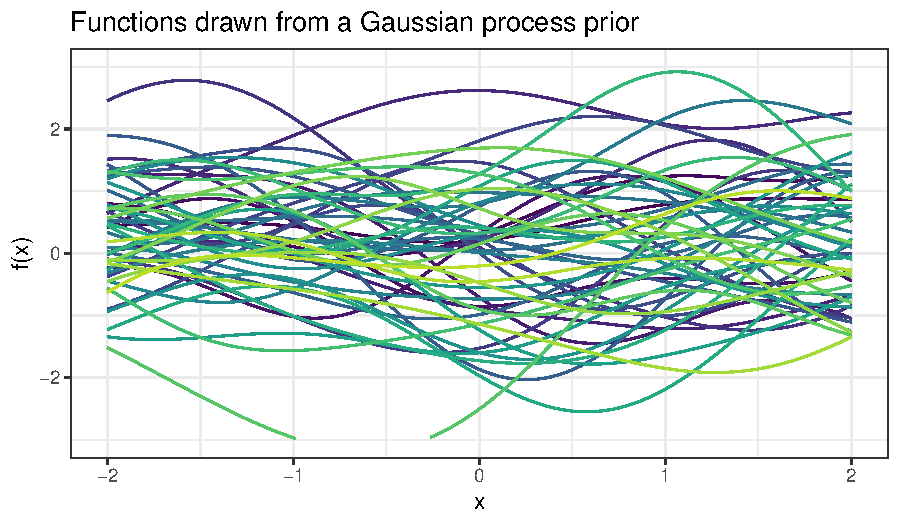
\includegraphics[width=0.7\textwidth]{figure/gp-prior} \\
\end{minipage}%
\begin{minipage}[b]{0.5\textwidth}
\centering
  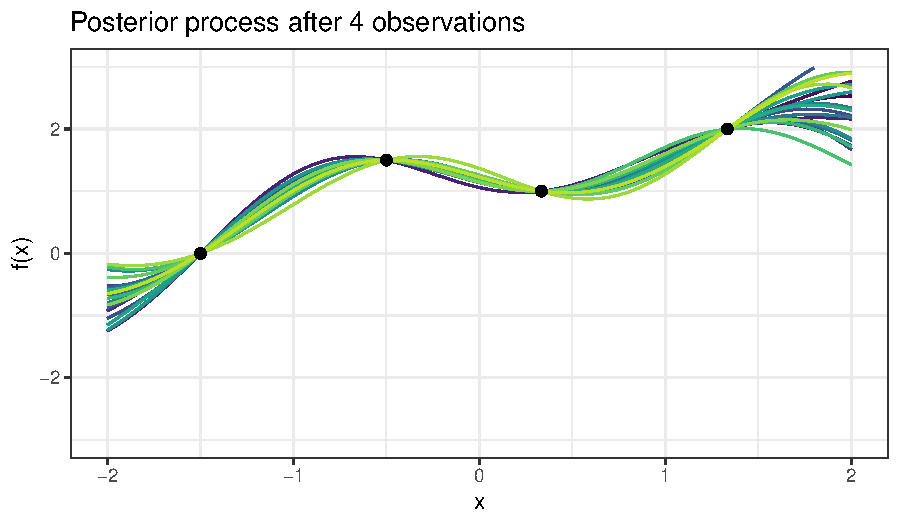
\includegraphics[width=0.7\textwidth]{figure/gp-posterior}
\end{minipage}

\end{frame}

% ------------------------------------------------------------------------------

\begin{frame}{Gaussian Processes (GP) -- method summary}
    
    \highlight{Empirical risk}
    \begin{itemize}
        \item The risk is estimated by using the posterior of a conditional Normal distribution
        \item Most kernels have \textbf{length scale parameters} that need to be estimated
    \end{itemize}
    \highlight{Optimization}
    \begin{itemize}
        \item The kernel parameters can be learned using \textbf{maximum likelihood} estimation
        \item This requires inverting the $n\times n$ -covariance matrix
    \end{itemize}
    \highlight{Hyperparameters}
    \begin{itemize}
        \item The most important hyperparameter is the choice of the kernel function $k(\xi, \xv^{(j)})$
        \item Common kernel choices for \textit{"standard"} data are:
        \begin{itemize}
            \item Linear or polyomial
            \item Squared-exponential (infinitely differentiable)
            \item Matérn (further generalization of the Squared-exponential kernel)
        \end{itemize}
        \item Special kernels for all kind of data situation exist, e.g., a Exp-Sine-Squared kernel for periodic data
        \item Kernels can be composed by multiplying or addition to create more expressive structures
    \end{itemize}
    
\end{frame}

% ------------------------------------------------------------------------------

\begin{frame}{Gaussian Processes (GP) -- Implementation \& Practical hints}

\highlight{Scalable GPs for larger data}
\begin{itemize}
	\item Low-rank approximations of the covariance by using only a representative subset of \textbf{inducing points}
	\item Using a kernel that creates a sparse coviariance matrix
\end{itemize}

\medskip

\highlight{Noisy GPs}
\begin{itemize}
    \item Having an interpolator might not be suitable if the data is noisy
    \item A noisy GP adds a \textbf{nugget} effect to the kernel $k(\xi, \xv^{(j)}) + \sigma\delta_{ij}$, creating a Gaussian process regression model
\end{itemize}

\medskip

\highlight{Implementation}

\begin{itemize}
  \item \textbf{R:} \texttt{mlr3} learners \texttt{LearnerClassifGausspr} /
    \texttt{LearnerRegrGausspr}, calling \texttt{kernlab::gausspr()}
  \item \textbf{Python:} \texttt{GaussianProcessClassifier} /
  \texttt{GaussianProcessRegressor} from package \texttt{scikit-learn}, \texttt{gpytorch} for a modular, scalable, efficient and GPU accelerated implementation built on \texttt{torch}
\end{itemize}

\end{frame}

\begin{frame}{Gaussian Processes (GP) -- Pros \& Cons}

\begin{columns}[onlytextwidth]
  \begin{column}{0.5\textwidth}
    \highlight{Advantages}
    \footnotesize
    \begin{itemize}
      \positem GPs allow to \textbf{quantify prediction uncertainty} induced by both intrinsic noise in the problem and errors in the parameter estimation process
      \positem A GP is a function \textbf{interpolator} and will predict the exact value of a training point
      \positem The choice of kernel function allows considerable flexibility for problem specific characteristics
      \positem Automatic relevance determination (ARD) determines the importance of features
      %\positem GP is \textbf{non-parametric} and can model virtually any functions of observations
    \end{itemize}
  \end{column}
  \begin{column}{0.5\textwidth}
    \highlight{Disadvantages}
    \footnotesize
    \begin{itemize}
      \negitem GPs are \textbf{not sparse}, i.e., they require the full training data for prediction
      \negitem GP training requires $\mathcal{O}(n^3)$, i.e., it scales cubically in the number of observations
      \negitem GPs cannot handle categorical features.
      \negitem GPs are \textbf{not particularly easy to understand} conceptually
    \end{itemize}
  \end{column}
\end{columns}

\end{frame}


\section{Neural Networks (NN)}


\begin{frame}{Neural Networks -- method summary}

% \maketag{un/SUPERVISED} 
\maketag{regression} \maketag{classification}
\maketag[50]{(non)parametric}
\maketag{BLACK-BOX} \maketag{feature selection}

\medskip

\highlight{General idea}
\begin{itemize}
  \item Learn \textbf{composite function} through series of nonlinear feature 
  transformations, represented as \textbf{neurons}, organized hierarchically 
  in \textbf{layers}
  \begin{itemize}
    \item Basic neuron operation: 1) affine \textbf{transformation} $\phi$ (weighted sum of inputs), 
    % multiplying inputs with weights (possibly including bias term), 
    2) nonlinear \textbf{activation} $\sigma$
    % , applying (nonlinear) function to transformed inputs
    \item Combinations of simple building 
    blocks to create a complex model
  \end{itemize}
  \item Optimize via \textbf{mini-batch stochastic gradient descent (SGD)} variants:
  \begin{itemize}
    \item Gradient of each weight can be infered from the \textbf{computational graph} of the network\\
    $\rightarrow$ \textbf{Automatic Differentiation} (AutoDiff)
    \item Algorithm to compute weight updates based on the loss is called \textbf{Backpropagation}
    %\textbf{Forward pass}: predict result with current parameters and 
    %compute empirical risk 
    %\item \textbf{Backward pass}: update each parameter in proportion to its 
    %error contribution $\Rightarrow$ gradients
  \end{itemize}
\end{itemize}

\medskip
 
\highlight{Hypothesis space} ~~
$\Hspace = \left\{ \fx: \fx = \tau \circ \phi \circ \sigma^{(h)} \circ
\phi^{(h)} \circ \sigma^{(h - 1)} \circ \phi^{(h - 1)} \circ ... \circ 
\sigma^{(1)} \circ \phi^{(1)} (\xv) \right\}$

\smallskip
\begin{center}
\begin{minipage}[b]{0.24\textwidth}
  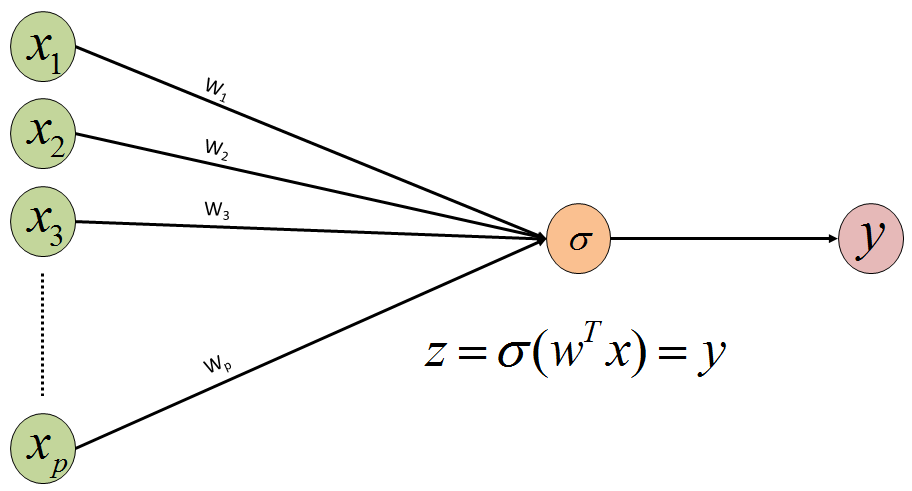
\includegraphics[width=0.9\textwidth]{figure/nn-single-neuron} \\
  %\tiny{Single neuron}
\end{minipage}%
\begin{minipage}[b]{0.24\textwidth}
  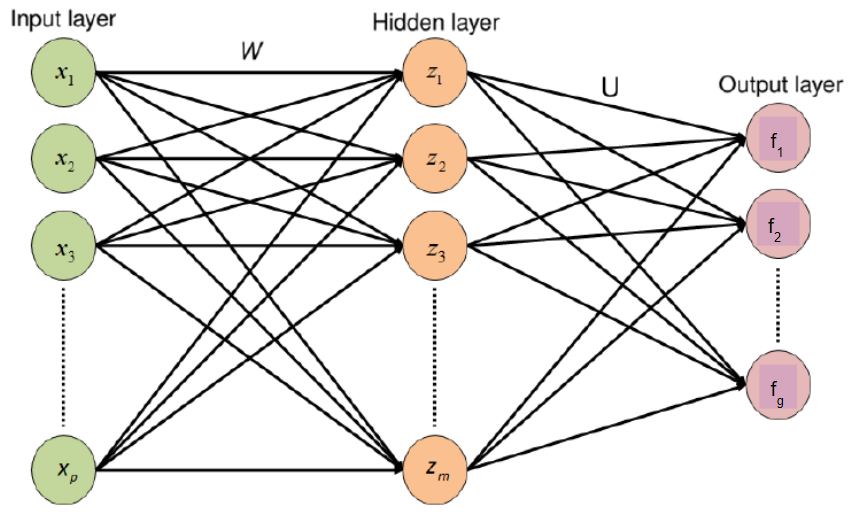
\includegraphics[width=0.9\textwidth]{figure/nn-feedforward} \\
  %\tiny{(Fully-connected) Feedforward network, 1 hidden layer}
\end{minipage}%
\end{center}


\end{frame}

% ------------------------------------------------------------------------------

\begin{frame}{Neural Networks -- method summary}

\footnotesize

\highlight{Architecture}

\begin{itemize}
    \item Input layer: original features $\xv$
    \item Hidden layers: nonlinear transformation of previous layer $\phi^{(h)} = \sigma^{(h - 1)}(\phi^{(h-1)})$
    \item Output layer: number of output neurons and activation depends on problem $\tau(\phi)$
    \begin{itemize}
    \item Regression: one output neuron, $\tau = $ identity
    \item Binary classification: one output neuron, $\tau = \frac{1}{1 + \exp(- \thx)}$ (logistic sigmoid)
    \item Multiclass Classification: $g$ output neurons, $\tau_j = \frac{\exp(f_j)}{\sum_{j=1}^g \exp(f_j)}$ (softmax)
\end{itemize}
\end{itemize}


\highlight{Empirical risk} In general, compatible with any differentiable loss

\medskip

\highlight{Optimization}

\begin{itemize}
  \item Variety of different optimizers, mostly based on some form of 
  \textbf{stochastic gradient descent (SGD)}\\
  \item Improvements: 
    \begin{itemize}
        \item[(1)] Accumulation of previous gradients $\rightarrow$ \textbf{Momentum}
        \item[(2)] Weight specific scaling based on previous squared gradients $\rightarrow$ \textbf{RMSProb}\\
        $\Rightarrow$ \textbf{ADAM} combines (1) and (2) 
        \item[(3)] Learning rate schedules, e.g., decaying or cyclical learning rates
    \end{itemize}
    \item Training progress is measured in full passes over the full training data, called \textbf{epochs}
    \item \textbf{Batch size} is a hyperparameter and limited by input data dimension
  % \item Crucial role of \textbf{regularization} due to high expressivity of 
  % NNs' hypothesis spaces
\end{itemize}

\end{frame}

% ------------------------------------------------------------------------------

\begin{frame}{Neural Networks -- method summary}

\highlight{Network types} ~~ Large variety of architectures for different data modelities
\begin{itemize}
  \item \textbf{Feedforward NNs / multi-layer perceptrons (MLPs):} sequence of 
  \textbf{fully-connected} layers $\Rightarrow$ tabular data
  \item \textbf{Convolutional NNs (CNNs):} sequence of feature map extractors 
  with spatial awareness $\Rightarrow$ images, time series
  \item \textbf{Recurrent NNs (RNNs):} handling of sequential, variable-length 
  information $\Rightarrow$ times series, text, audio
  \item \textbf{Transformers:} Learning invariances from data, handling multiple/any data modalities
  %\item Unsupervised: \textbf{autoencoders}, \textbf{generative adversarial networks (GANs)}, \dots
  % \item \textbf{Autoencoders:} learning unsupervised embeddings
  % \item \textbf{Generative adversarial networks (GANs):} learning to generate 
  % artificial samples
\end{itemize}

\begin{minipage}[b]{0.49\textwidth}
\begin{center}
  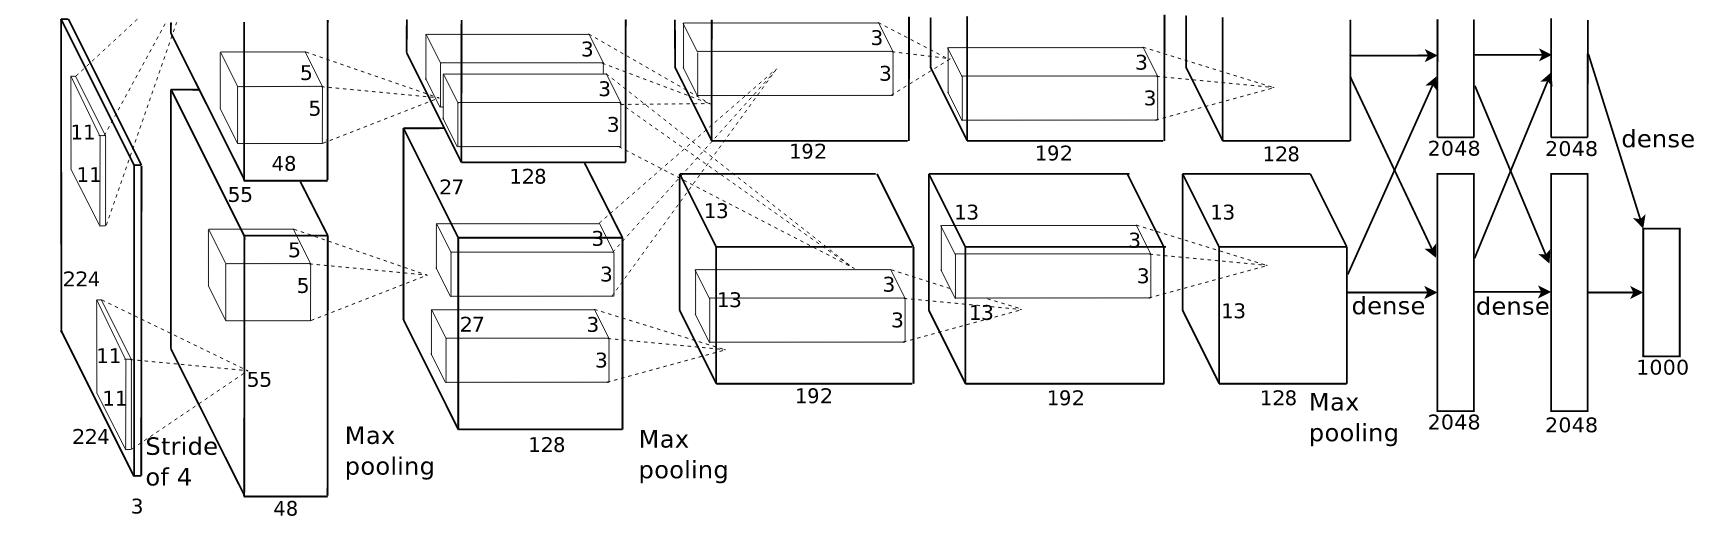
\includegraphics[width=.9\textwidth]{figure/nn-cnn-1} \\
  \tiny{Convolutional network architecture}\\ \medskip
  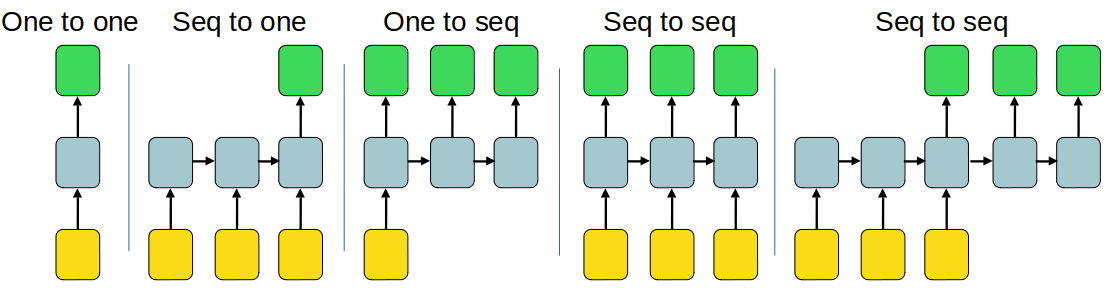
\includegraphics[width=.9\textwidth]{learners-overview/figure/one_to_one.png} \\
  \tiny{Recurrent network architecture}
\end{center}
\end{minipage}
\begin{minipage}[b]{0.49\textwidth}
\begin{center}
  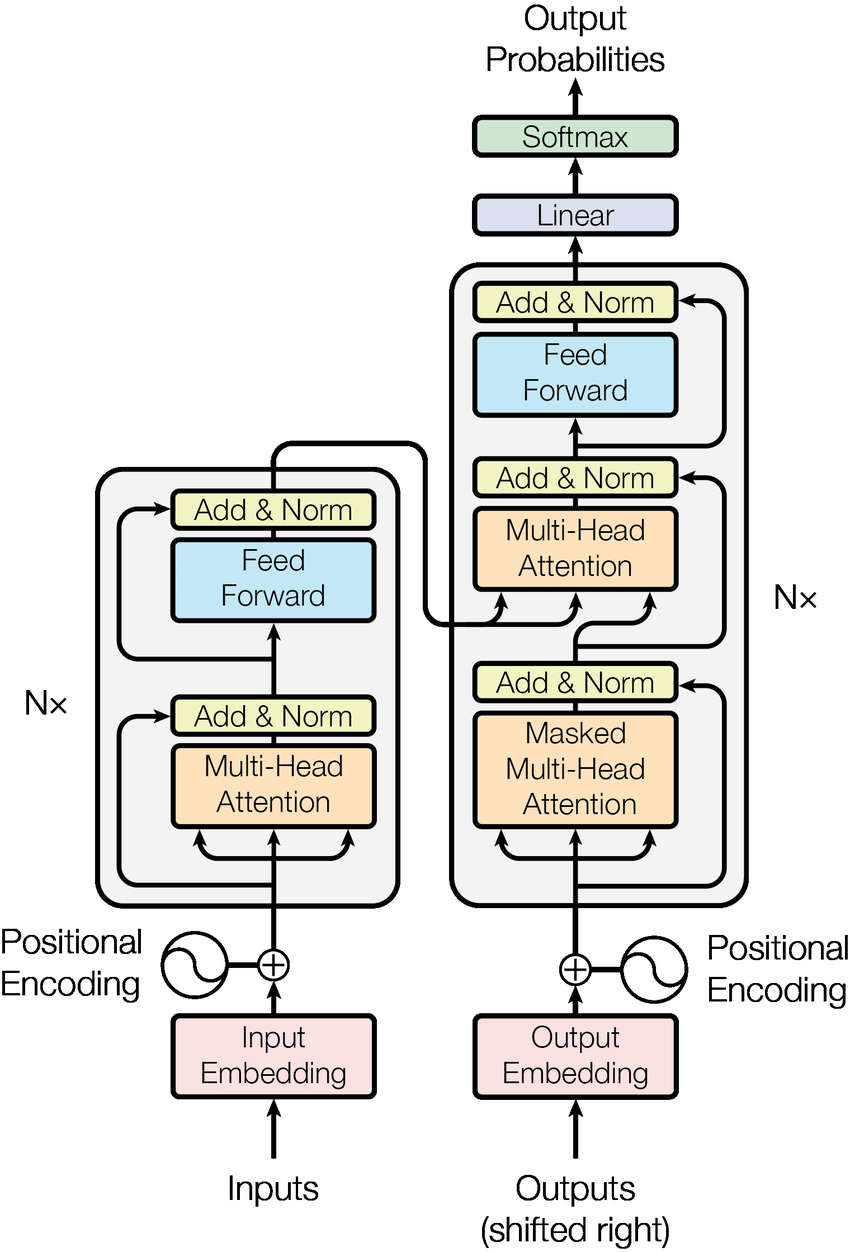
\includegraphics[width=.4\textwidth]{learners-overview/figure/transformer.png} \\
  \tiny{Transformer network architecture}
\end{center}
\end{minipage}

\end{frame}

% ------------------------------------------------------------------------------

\begin{frame}{Neural Networks -- method summary}

\footnotesize


\highlight{Hyperparameters}

\begin{itemize}
  \item \textbf{Architecture}:
  \begin{itemize}
    \item Lots of design choices $\Rightarrow$ tuning problem of its own.
    \item Typically: hierachical optimization of components (cells) and macro structure of network\\ 
    $\rightarrow$ \textbf{Neural Architecture Search (NAS)}
    \item Many predifined (well working) architectures exist for standard tasks
  \end{itemize}
  \item \textbf{Training}:
  \begin{itemize}
    \item Initial learning rate and various regularization parameters
    \item Number of epochs is determined by \textbf{early-stopping}
    \item \textbf{Data-augmentation}, e.g., applying random rotations to input images
    %Crucial due to \textbf{overparameterization} and strong 
    %\textbf{nonconvexity} 
    %\item E.g., weight initialization, choice of optimizer, learning rate, 
    %batch size, number of epochs, \dots
  \end{itemize}
\end{itemize}

\medskip

\highlight{Foundation models}

\begin{itemize}
    \item \textbf{Enormous} models trained on vast amounts of (general) data, e.g., all of wikipedia, in \textbf{self-supervised} fashion
    \item Used as starting point (\textbf{pre-trained}) and fine-tuned via \textbf{transfer} or \textbf{few-shot} learning for other tasks requiring little data
    \item Examples: GPT-3 for language, CLIP for vision-language, \dots
\end{itemize}

%\begin{itemize}
%    \item Makes choice of the architecture dispensable\\
%          $\Rightarrow$ Pre-defined architecture with pre-trained weights is used
%    \item Reduces training cost a lot, since pre-trained weights are only adapted during fine-tuning
%    \item \textbf{Pre-training} done in a self-supervised fashion on ubiquituous amount of data\\
%          $\Rightarrow$ In self-supervised learning, labels are generated from the data itself, no human labeling effort needed
%\end{itemize}

% \highlight{Runtime behavior} ~~ \textcolor{blue}{???}

\end{frame}


% ------------------------------------------------------------------------------

\begin{frame}{Neural Networks -- Implementation \& Practical hints}

\highlight{General hints}
\begin{itemize}
    \item Instead of NAS, use a standard architecture and tune training hyperparameters
    \item Training pipeline (data-augmentation, training schedules, ...) is more crucial than the specific architecture
    \item While NNets are state-of-the-art for \textbf{computer vision (CV)} and \textbf{natural language processing (NLP)}, we recommend not to use them for tabular data because alternatives perform better
    \item Computational efforts for training (and inference) can be very high, requiring specific hardware.\\
    $\rightarrow$ Using a service (esp. for foundation models) can be more cost efficient
\end{itemize}

%\highlight{Some options for regularization} 
%\begin{itemize}
%  \item Control weight magnitude with \textbf{weight decay} (L2 
%  regularization)
%  \item Interrupt training when validation error starts to pick up 
%  $\Rightarrow$ \textbf{early stopping}
%  \item Use \textbf{dropout} to deactivate neurons at random, thus down-sizing 
%  network
%  \item Expand training data and enforce invariances via \textbf{augmentation}
%  \item \dots
%\end{itemize}

%\highlight{Optimization tricks}
%\begin{itemize}
%  \item Accelerate training via optimizer (ADAM, Momentum)
%  \item Control learning rate with \textbf{schedulers}, or keep it 
%  \textbf{adaptive}
%  \item Use \textbf{batch normalization} for stability by keeping input distributions fixed throughout transformations
%  \item \dots
%\end{itemize}

% \highlight{Types of neural networks (RNNs, CNNs)}
% 
% \begin{itemize}
%   \item \textbf{Recurrent neural networks (RNNs}: Deep NN that make use of 
%   \textbf{sequential} information with temporal \textbf{dependencies} \\
%   $\rightarrow$ Frequently applied to \textbf{natural language processing}
%   \item \textbf{Convolutional neural networks (CNNs)}: Regularized version of the 
%   fully connected feed-forward NN (where each neuron is connected to all 
%   neurons of the subsequent layer) that abstracts inputs to feature maps via 
%   \textbf{convolution} \\
%   $\rightarrow$ Frequently applied to \textbf{image recognition}
% 
% \end{itemize}
% 
% \medskip
% 
% \highlight{Problem of neural architecture search (NAS)}
% 
% NN are \textbf{not off-the-shelf} methods -- the network architecture needs to 
% be tailored to each problem anew \\
% $\rightarrow$ Automated machine learning attempts to learn architectures

\medskip
 
\highlight{Implementation}

\begin{itemize}
  \item \textbf{R:} Use python libraries (below) via \texttt{reticulate}, but not really recommended except for toy applications.
  \item \textbf{Python libraries:} 
  \begin{itemize}
      \item \texttt{keras} for simple high level API 
      \item \texttt{PyTorch} for flexible design with a focus on research
      \item \texttt{TensorFlow} for flexible design with a focus on deployment / industry
      \item \texttt{huggingface} for pre-trained / foundation models
  \end{itemize}
\end{itemize}

\end{frame}


% ------------------------------------------------------------------------------

\begin{frame}{Neural Networks -- Pros \& Cons}

\footnotesize

\begin{columns}[onlytextwidth]
  \begin{column}{0.5\textwidth}
    \highlight{Advantages}
    \footnotesize
    \begin{itemize}
      \positem Applicable to \textbf{complex, nonlinear} problems
      \positem Very \textbf{versatile} w.r.t. architectures
      \positem State-of-the-art for CV and NLP
      \positem Strong \textbf{performance} if done right
      \positem Built-in \textbf{feature extraction}, obtained by intermediate
      representations
      \positem Easy handling of \textbf{high-dimensional} data
      \positem \textbf{Parallelizable} training 
    \end{itemize}
  \end{column}

  \begin{column}{0.5\textwidth}
    \highlight{Disadvantages}
    \footnotesize
    \begin{itemize}
      \negitem Typically, high computational \textbf{cost}
      \negitem High demand for \textbf{training data} 
      \negitem Strong tendency to \textbf{overfit}
      \negitem Requiring lots of \textbf{tuning expertise} 
      \negitem \textbf{Black-box} model -- hard to interpret or explain
    \end{itemize}
  \end{column}
\end{columns}

\end{frame}

\endlecture

\end{document}
